%%%%%%%%%%%%%%%%%%%camp

\section*{Einleitung}

\begin{frame}
    \frametitle{Antenne}
      \begin{center}
        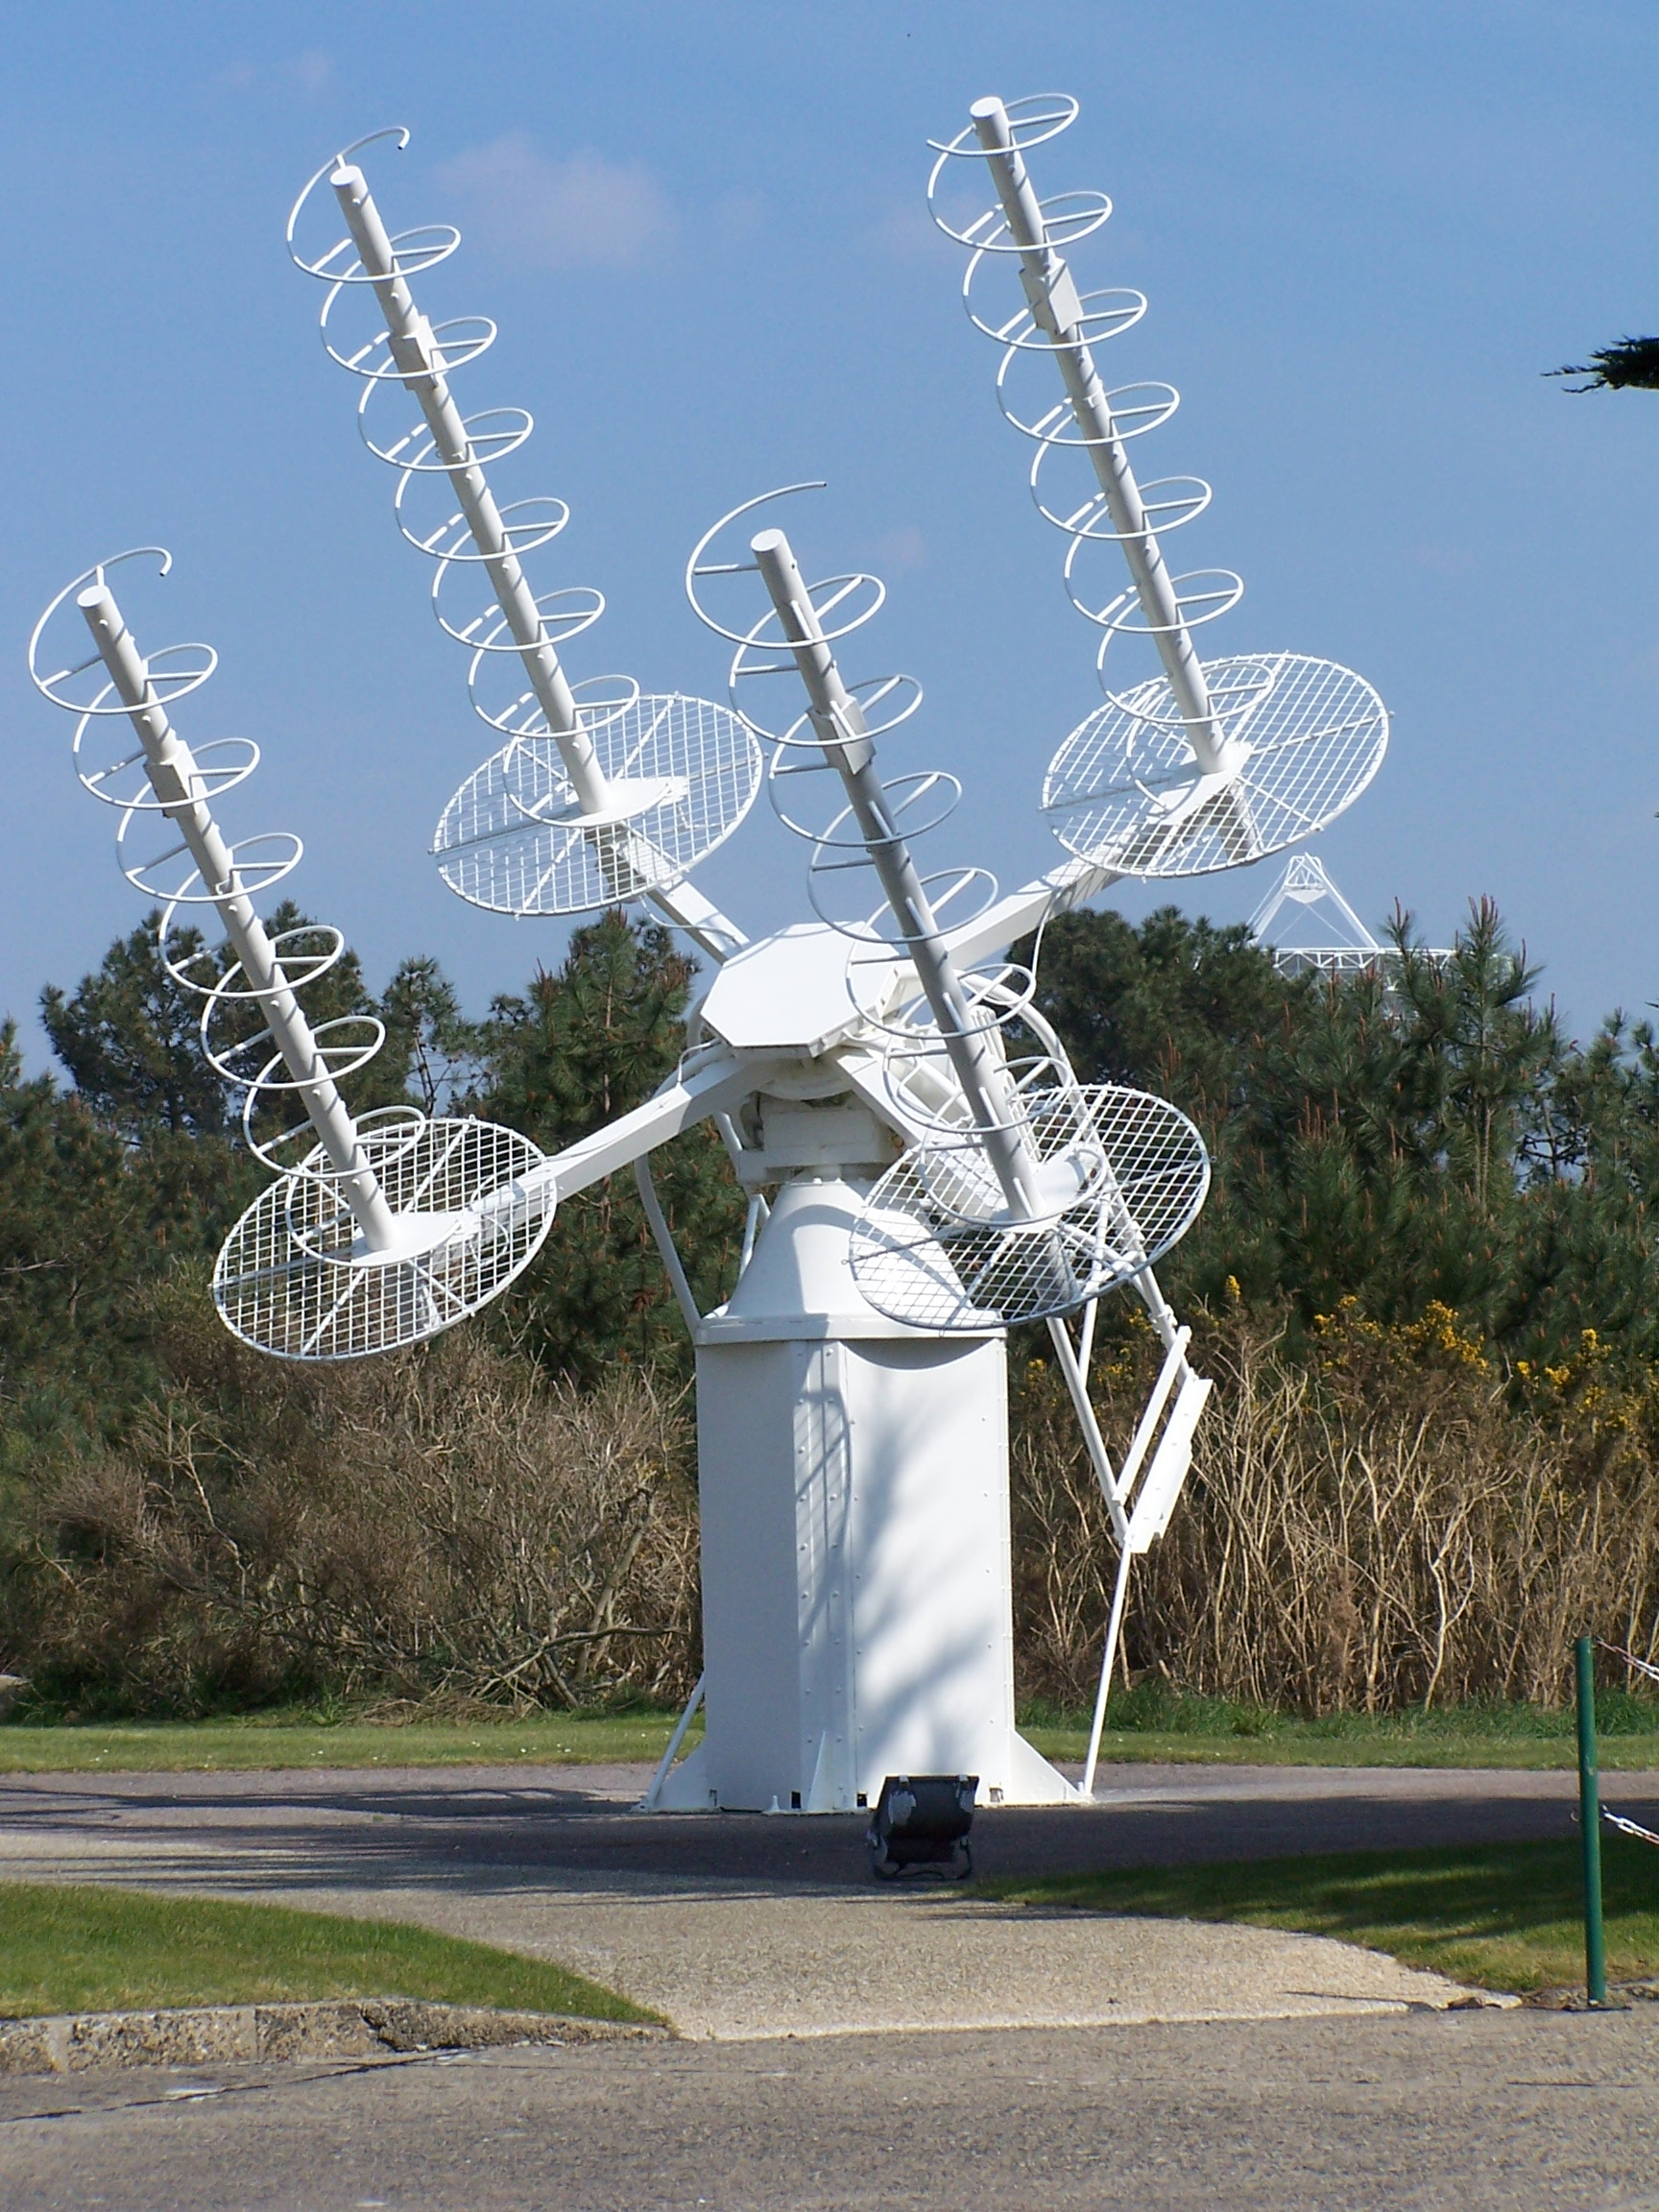
\includegraphics[width=.5\textwidth]{e11/Traqueur_acquisition.JPG}
        \footnote{\tiny \url{https://upload.wikimedia.org/wikipedia/commons/3/32/Traqueur_acquisition.JPG}}
    \end{center}
\end{frame}
  
\begin{frame}
	\frametitle{Einleitung}
\begin{minipage}{0.49\textwidth}
	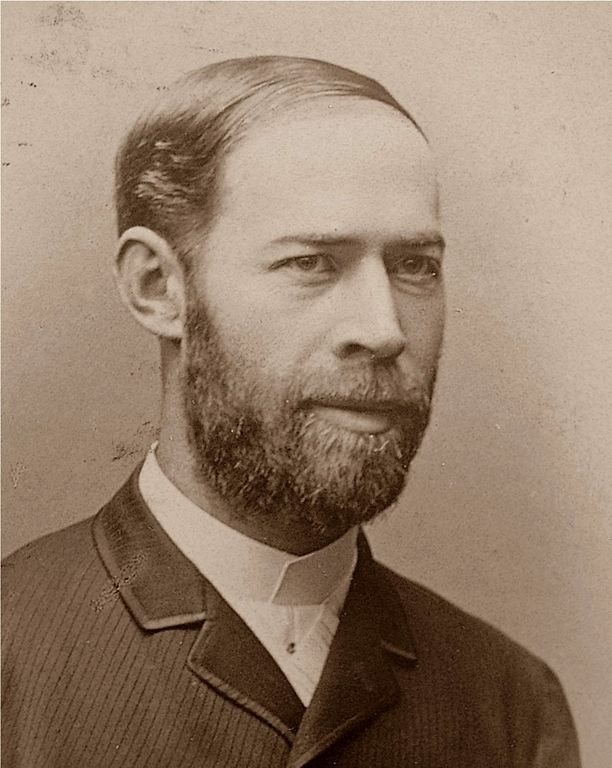
\includegraphics[width=1\textwidth]{antennen101/HEINRICH_HERTZ.jpg}
	\tiny \hyperlink{refs}{\cite{wc}}
\end{minipage}
\begin{minipage}{0.49\textwidth}
	\begin{itemize}
		\item Heinrich Hertz (1851-1894)
		\item Nachweis Elektromagnetischer Wellen 1888	
		\item Herzscher Dipol
	\end{itemize}
\end{minipage}
\end{frame}

\begin{frame}
    \frametitle{Schwingkreis}
    \begin{center} \huge
    $$f = \frac{1}{2  \pi \cdot \sqrt{LC}}$$
        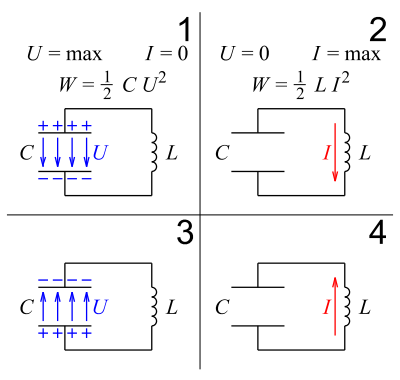
\includegraphics[width=.8\textwidth]{antennen101/Schwingkreis.png}
	\end{center}
\end{frame}


\begin{frame}
    \frametitle{Dipol}
    \begin{center}
        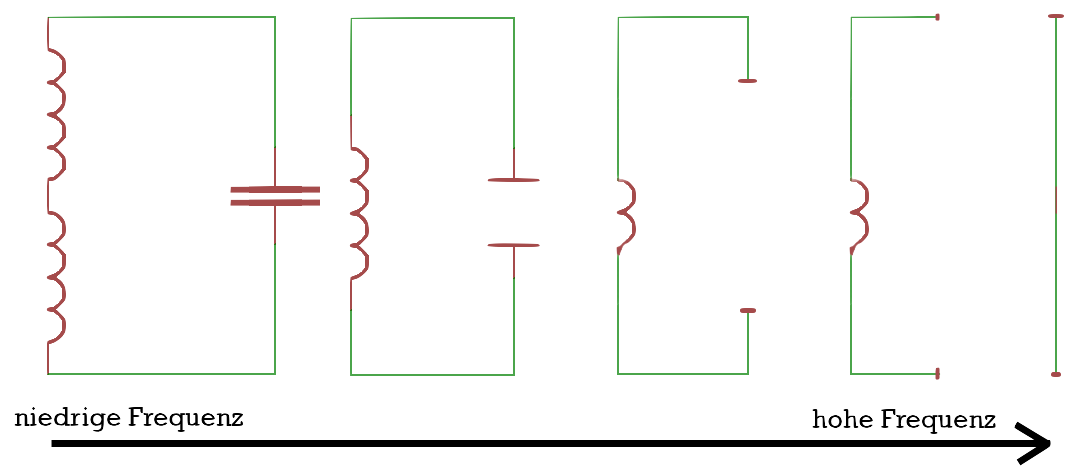
\includegraphics[width=1\textwidth]{e11/dipol_entstehung.png}
        \footnote{\tiny by DB4UM}
	\end{center}
\end{frame}

\begin{frame}
    \frametitle{E- und H-Feld}
    \begin{center}
        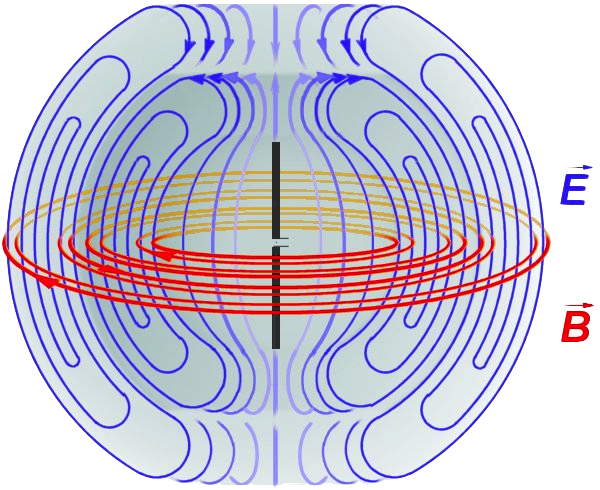
\includegraphics[width=0.85\textwidth]{e11/Felder_um_Dipol.png}
        \footnote{\tiny \url{https://commons.wikimedia.org/wiki/File:Felder_um_Dipol.jpg}}
	\end{center}
\end{frame}


\section*{Dipol}

\begin{frame}
    \frametitle{Dipol}
    \begin{center}
        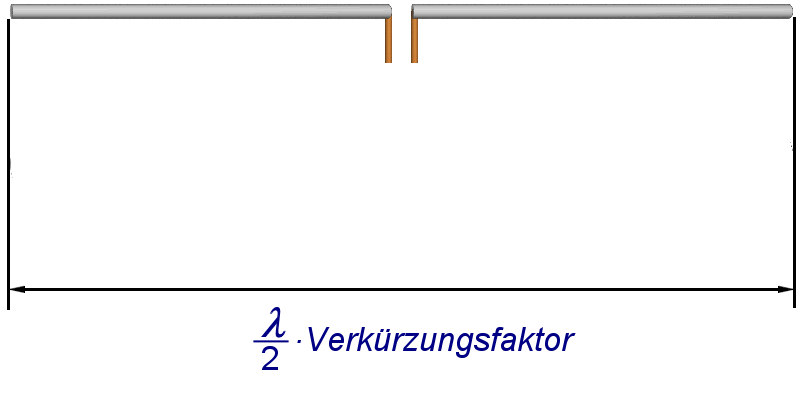
\includegraphics[width=1\textwidth]{antennen101/Faltdipol.png}
        \footnote{\tiny \url{https://commons.wikimedia.org/wiki/File:Faltdipol.png}}
	\end{center}
\end{frame}


\begin{frame}
    \frametitle{Wellenlänge}
    \begin{center} \huge
        $$\lambda = \frac{c}{f}$$
      	mit $c = 299\,792\,458 ~ \mathrm{m/s}$
	\end{center}
\end{frame}

\begin{frame}
    \frametitle{Wellenlänge einfacher}
    \begin{center} \huge
        $$\lambda [m] = \frac{300}{f[MHz]}$$
	\end{center}
\end{frame}

\begin{frame}
    \frametitle{$\lambda / 2$ Dipol berechnen}
    \begin{center}
	\begin{itemize} \Large
		\item Theoretische Strahlerlänge eines $\lambda / 2$ Dipols für 7MHz berechnen
		\item $\lambda[m] = \frac{300}{f[MHz]}$
    \end{itemize}
    \end{center}
\end{frame}

\begin{frame}
    \frametitle{Verkürzungsfaktor beachten}
    \begin{center}
	\begin{itemize} \Large
		\item Inerhalb von Feststoffen breiten sich EM-Wellen nicht mit Lichtgeschwindigkeit aus.
		\item Deshalb: $\lambda[m] = \frac{300}{f[MHz]} \cdot $ Verkürzungsfaktor
		\item z.B. bei Kupfer $0.95$
    \end{itemize}
    \end{center}
\end{frame}

\begin{frame}
    \frametitle{Fertig?}
    \begin{center}
        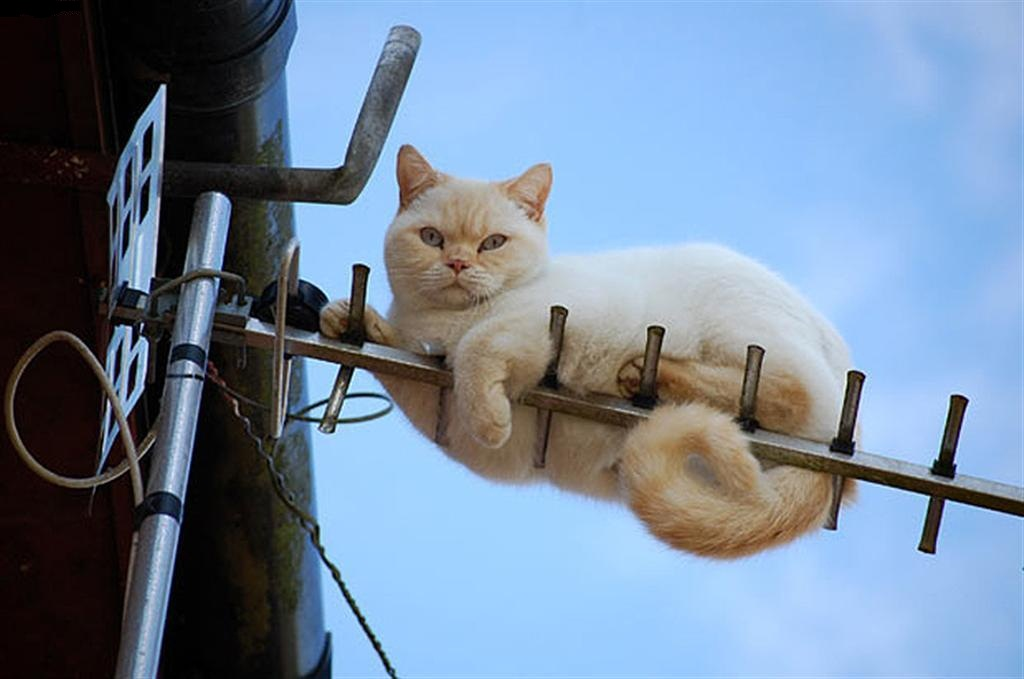
\includegraphics[width=.95\textwidth]{antennen101/cat-antenna.jpg}
        \footnote{\tiny \url{http://www.socalgreenrealestateblog.com/control-your-homes-energy-use-with-these-apps/cat-antenna/}}
	\end{center}
\end{frame}

\begin{frame}
    \frametitle{Strom und Spannungsverteilung}
	\begin{itemize}
		\item Stahlerlänge $\lambda / 2$
		\item Stromknoten und Spannungsbauch an den Enden (Unendlich großer Widerstand)
        \item Spannung nicht überall gleich groß
    \end{itemize}
    \begin{center}
        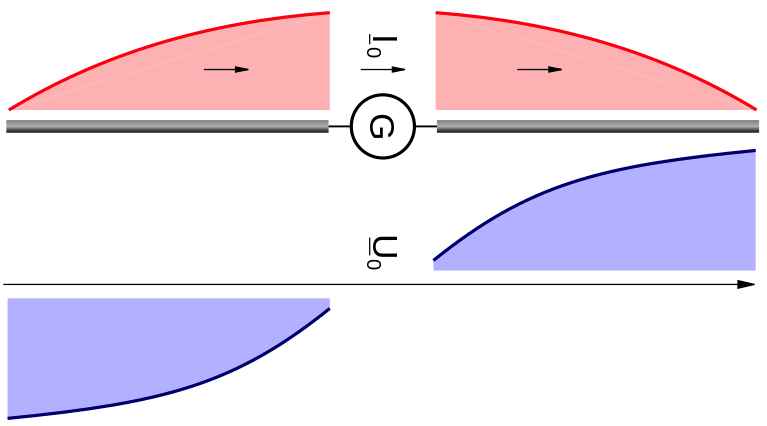
\includegraphics[width=0.85\textwidth]{e11/DipolUI.png}
        \footnote{\tiny \url{https://commons.wikimedia.org/wiki/File:Lineare_antennen.svg}}
	\end{center}
\end{frame}

\begin{frame}
    \frametitle{Fußpunktwiderstand}
    \begin{center}
	\begin{itemize}
		\item Fußpunktwiderstand/Impedanz/Speisewiderstand
		\item Beim Dipol im freien Raum: $70 \Omega$
		\item je nach Dipolhöhe zwischen $40  \Omega$ und $80  \Omega$
		\item  Bei $0.15 \lambda$ Höhe $50  \Omega$ Speisewiderstand 
    \end{itemize}
 	\end{center}
\end{frame}

\begin{frame}
    \frametitle{Prüfungsfrage}
    \begin{center}
    \begin{tabular}{l||l}\hline
        TH206 & Ein Halbwellendipol wird auf der  \\
         " "  & Grundfrequenz in der Mitte \\ \hline\hline
         A & spannungsgespeist.\\\hline
         B & stromgespeist. \\\hline
         C & endgespeist. \\ \hline
         D & parallel gespeist.\\\hline
    \end{tabular}
 	\end{center}
\end{frame}

\begin{frame}
    \frametitle{Prüfungsfrage}

    \begin{center}
    \begin{tabular}{l||l}\hline
        TH206 & Ein Halbwellendipol wird auf der  \\
         " "  & Grundfrequenz in der Mitte \\ \hline\hline
         " " & spannungsgespeist.\\\hline
         X & stromgespeist. \\\hline
         " " & endgespeist. \\ \hline
         " " & parallel gespeist.\\\hline
    \end{tabular}
        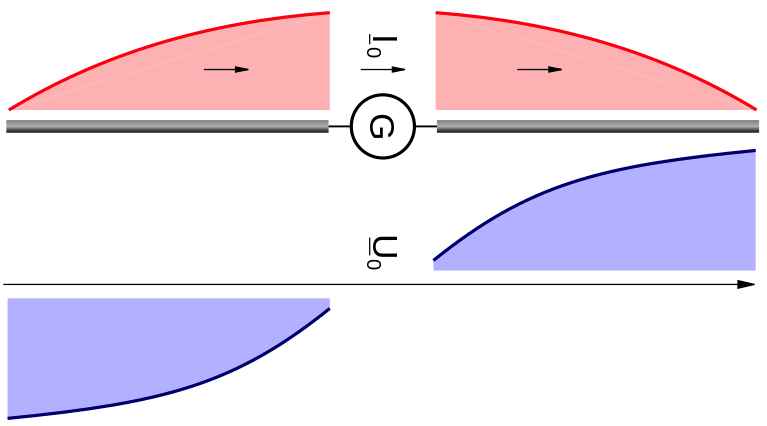
\includegraphics[width=0.85\textwidth]{e11/DipolUI.png}
        \footnote{\tiny \url{https://commons.wikimedia.org/wiki/File:Lineare_antennen.svg}}
 	\end{center}
\end{frame}


\begin{frame}
    \frametitle{Fußpunktwiderstand}
    \begin{center}
	\begin{itemize}
		\item Erwünschter Widerstand: Real $50 \Omega$ Imaginär $O \Omega$
		\item SWR-Meter (Standing wave Ratio) möglichst 1:1 ($S_{11} < -17$)
    \end{itemize}
 	\end{center}
\end{frame}

\begin{frame}
    \frametitle{SWR}
    \begin{center}
	\begin{itemize}
		\item Aussage über verhältnis Widerstand am Kabelende zu Widerstand an der Antenne
		\item Informationen darüber wie viel Leistung an die Antenne abgegeben wird
		\item Nicht an die Antenne gegebene Leistung wird zurück in die Endstufe reflektiert
		\item Keine Aussage über Abstrahleigenschaften der Antenne ($50 \Omega$ R ist perfekt)
		\item Typische Werte für eine reale Antenne im WLAN-Bereich liegen etwa bei 2:1 bis 2,5:1.
		\item Für rad1o werden Antennen benötigt mit SWR besser als 2:1
    \end{itemize}
 	\end{center}
\end{frame}

\begin{frame}
    \frametitle{Schwingkreis}
    \begin{center} \large
    Messung einer selbstgebauten Yagi für $10m$ bei DK0TU
        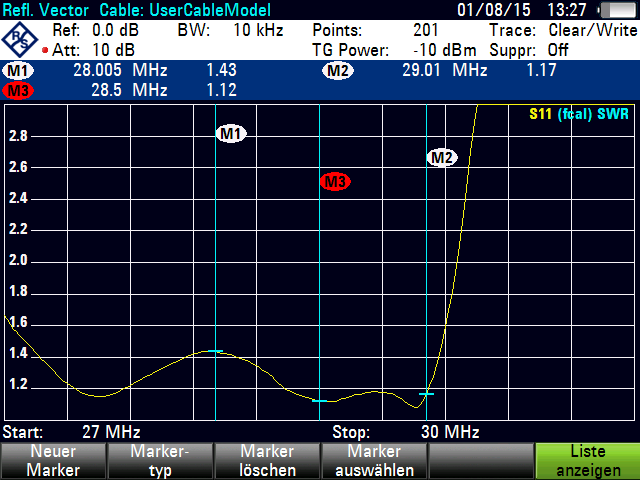
\includegraphics[width=.9\textwidth]{antennen101/Measurement0010.png}
	\end{center}
\end{frame}


\section*{Richtdiagramm}

\begin{frame}
    \frametitle{Richtdiagramm Dipol}
    \begin{center}
        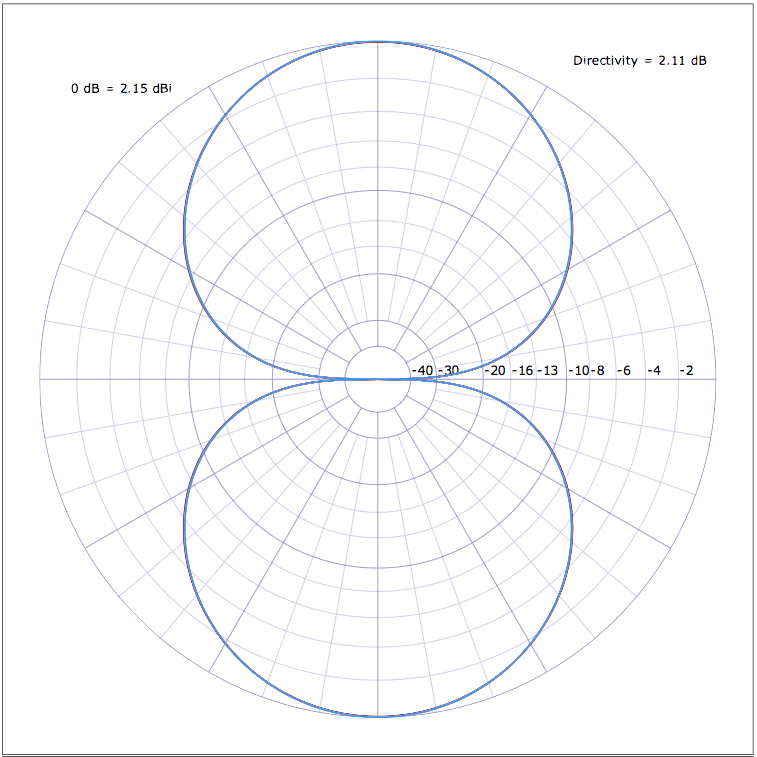
\includegraphics[width=0.75\textwidth]{e11/Richt-Dipol.png}
        \footnote{\tiny DB4UM Programm: cocoaNec 2.0}
	\end{center}
\end{frame}

\section*{Gewinn}

\begin{frame}
    \frametitle{EIRP und ERP}
    \begin{itemize}
    	\item ERP
		    \begin{itemize}
				\item Effektive Radiated Power
       		 	\item Bezug auf Dipol
       		 	\item $P_{ERP} = G_{Dipol} \cdot (P_{Sender} - P_{Verlust})$
 		   	\end{itemize}
		\item EIRP
		    \begin{itemize}
				\item Effektive Isotropic Radiated Power
       		 	\item Bezug auf Isotropstrahler
       		 	\item $dB_{ERP} = 2.15 + dB_{EIRP}$
       		 	\item $P_{EIRP} = 1.64 \cdot P_{ERP}$
 		   	\end{itemize}
    \end{itemize}
\end{frame}

\begin{frame}
    \frametitle{Isotropstrahler}
    \begin{center}
        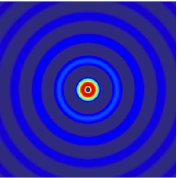
\includegraphics[width=0.75\textwidth]{e11/Spherical_wave2.png}
        \footnote{\tiny \url{https://commons.wikimedia.org/wiki/File:Spherical_wave2.gif}}
	\end{center}
\end{frame}

\section*{Multiband}

\begin{frame}
    \frametitle{Multiband Dipol}
    $2.15dBi$
    \begin{center}
        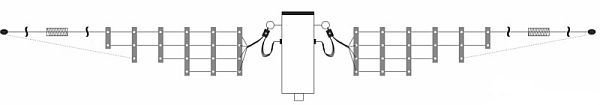
\includegraphics[width=0.9\textwidth]{e11/Multiband.jpg}
        \footnote{\tiny Antenne EA-1015204080 von EAntenna}
	\end{center}
\end{frame}


\section*{Yagi-Uda}

\begin{frame}
    \frametitle{Yagi-Uda}
    $5dBi$-$30dBi$
    \begin{center}
        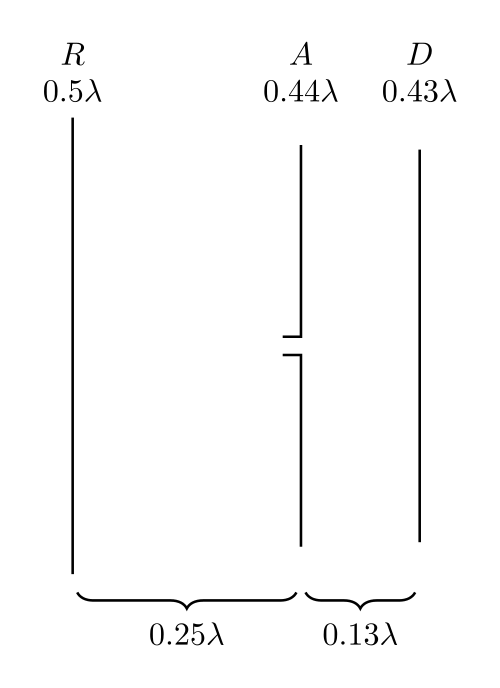
\includegraphics[width=0.5\textwidth]{e11/Yagi_3_element.png}
        \footnote{\tiny \url{https://commons.wikimedia.org/wiki/File:Yagi_3_element.svg}}
	\end{center}
\end{frame}


\begin{frame}
    \frametitle{Richtdiagramm Yagi}
    \begin{center}
        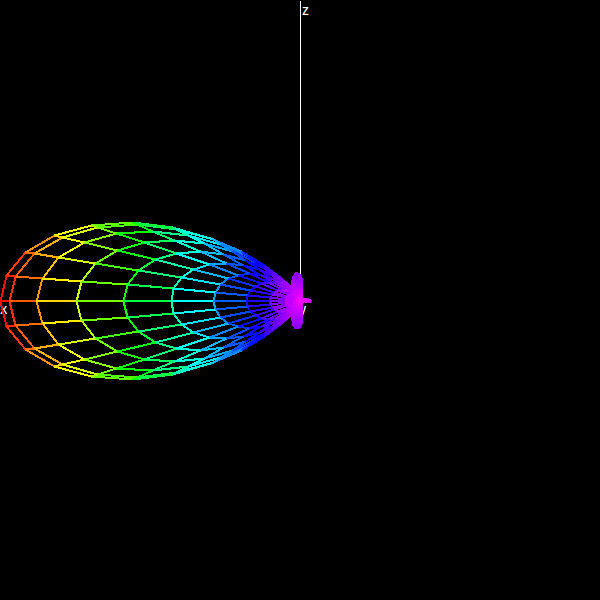
\includegraphics[width=0.7\textwidth]{e11/yagi_gain.png}
        \footnote{\tiny DK0TU 10m Yagi 28.1 MHz von DL2JAS Programm: EZNEC}
	\end{center}
\end{frame}

\begin{frame}
    \frametitle{Yagi - Richtung erkennen}
    \begin{center}
        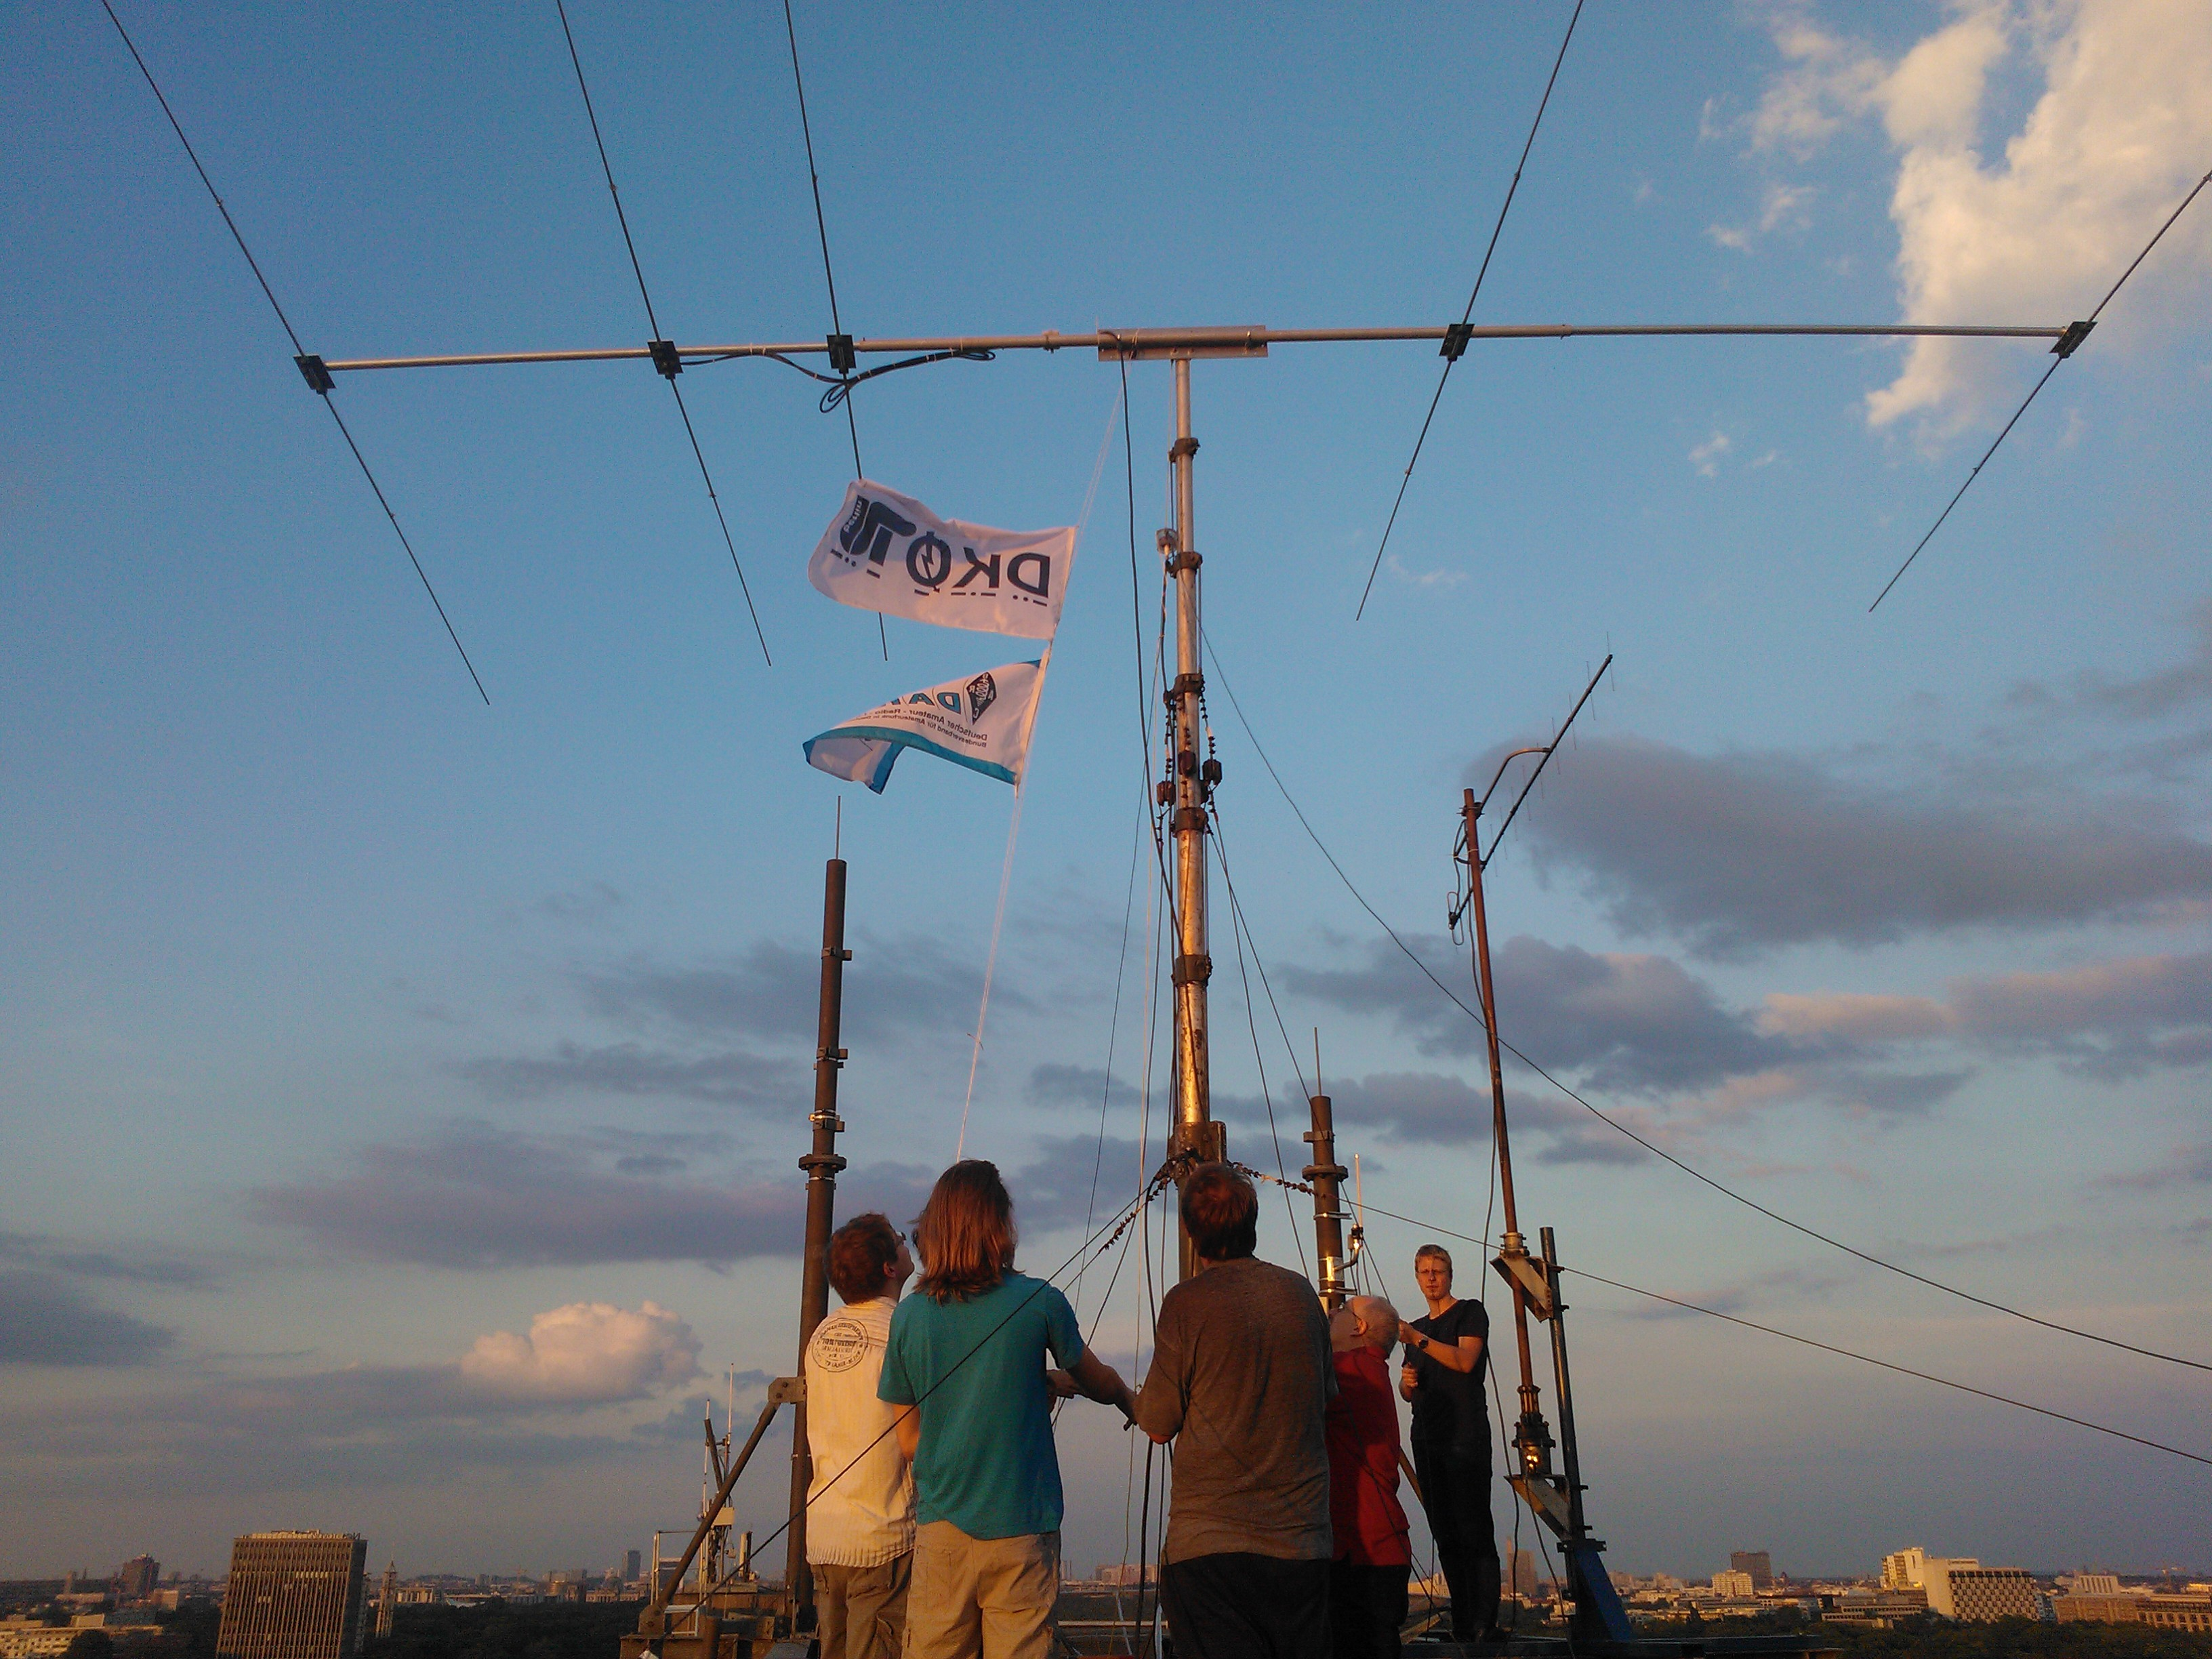
\includegraphics[width=.9\textwidth]{e11/yagi.jpg}
        \footnote{\tiny 10M Yagi bei DK0TU von DK9GD}
	\end{center}
\end{frame}


\section*{Groundplane}

\begin{frame}
    \frametitle{Groundplane}
    $2.15dBi$ - Jeder Draht $\lambda / 4$
    \begin{center}
        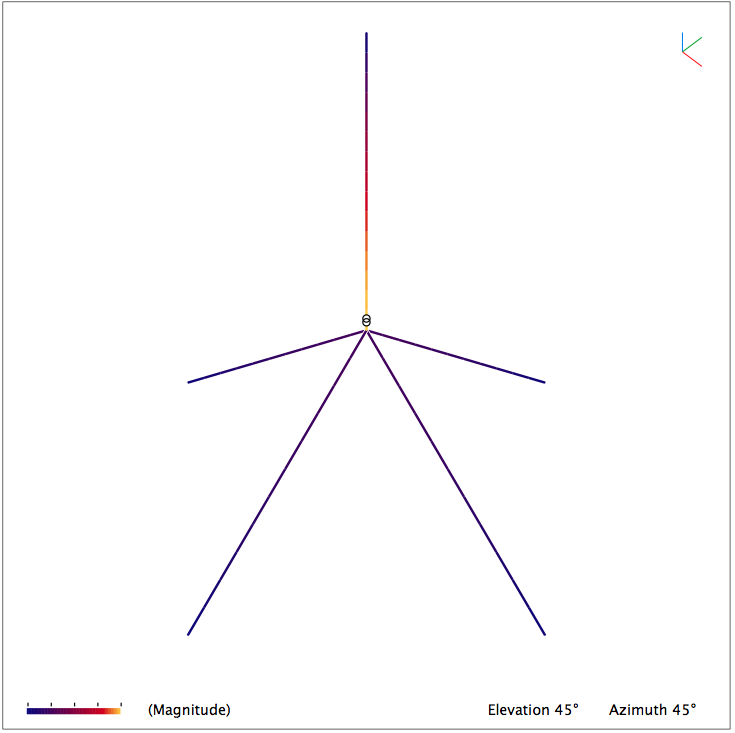
\includegraphics[width=0.7\textwidth]{e11/GP-DB4UM.png}
        \footnote{\tiny DB4UM mit cocoaNec 2.0}
	\end{center}
\end{frame}

\begin{frame}
    \frametitle{Spiegelladung}
    \begin{center}
        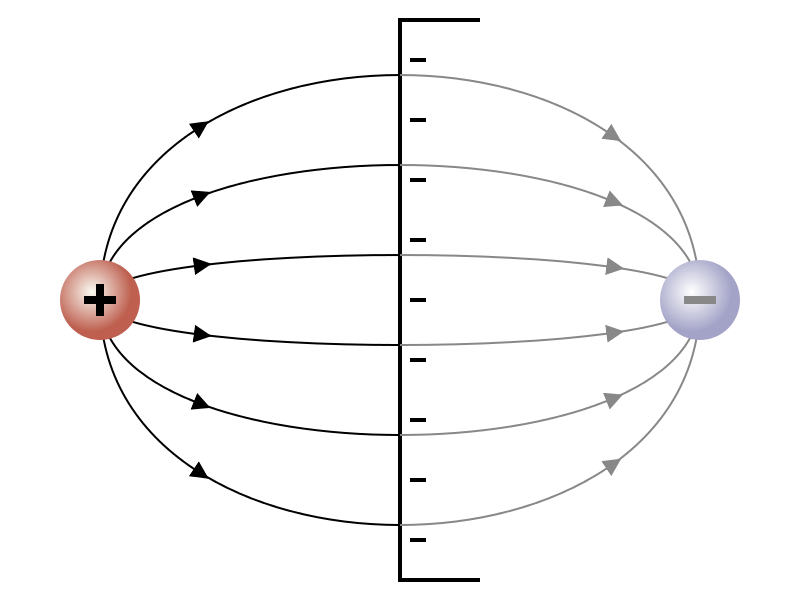
\includegraphics[width=0.7\textwidth]{antennen101/Spiegelladung.png}
                \footnote{\tiny \url{https://de.wikipedia.org/wiki/Datei:Spiegelladung.svg}}
	\end{center}
\end{frame}

\begin{frame}
    \frametitle{Spiegelladung}
    \begin{center}
        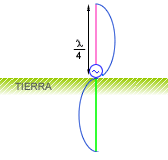
\includegraphics[width=0.7\textwidth]{antennen101/Antena_marconi501.png}
                \footnote{\tiny \url{https://de.wikipedia.org/wiki/Datei:Spiegelladung.svg}}
	\end{center}
\end{frame}

\begin{frame}
    \frametitle{Magnetfuss-Antenne}
    \begin{center}
        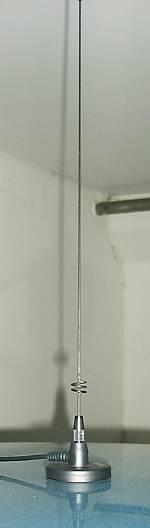
\includegraphics[height=0.99\textheight]{antennen101/magnetfuss.jpg}
                \footnote{\tiny \url{https://de.wikipedia.org/wiki/Datei:Spiegelladung.svg}}
	\end{center}
\end{frame}

\section*{Magnetic Loop}

\begin{frame}
    \frametitle{Magnetic Loop}
    \begin{center}
        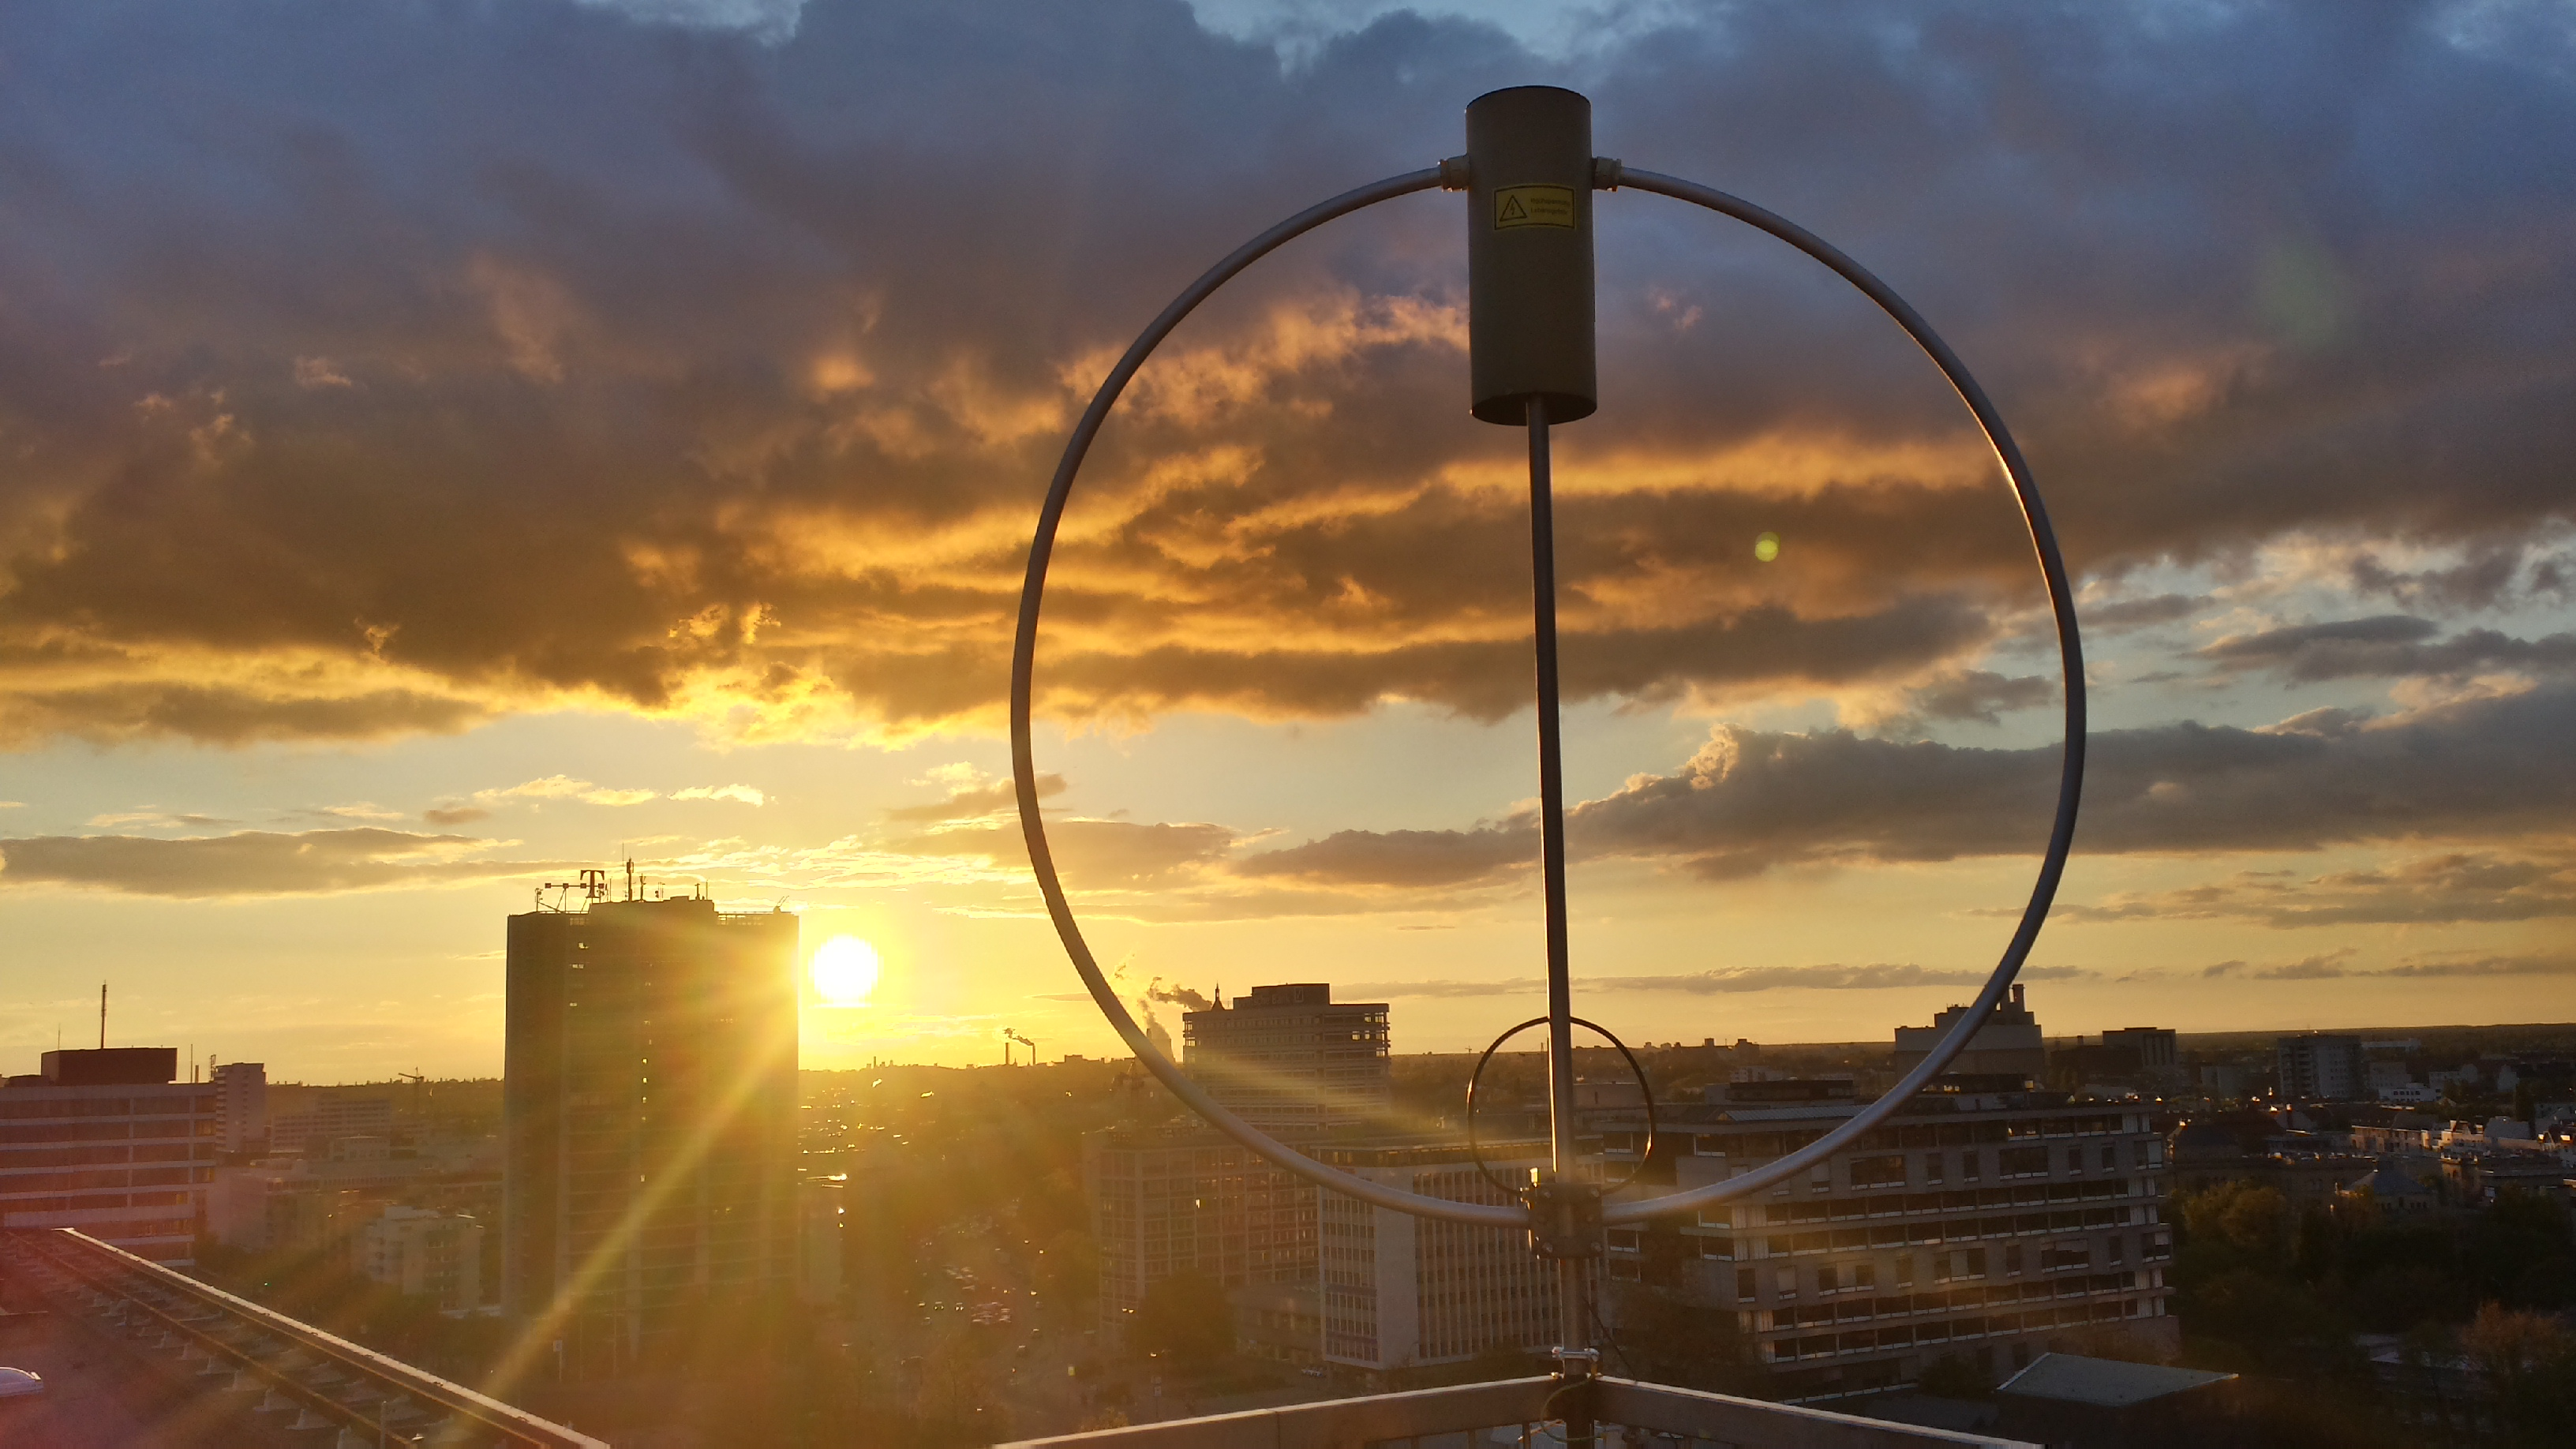
\includegraphics[width=1\textwidth]{e11/Magloop.jpg}
        \footnote{\tiny Magloop bei DK0TU von DB4UM}
	\end{center}
\end{frame}

\section*{Polarisierung}

\begin{frame}
    \frametitle{Polarisierung}
    	\begin{itemize}
		\item Antennen sind Vertikaloder Horizontal Polarisiert?
		\item Wie ist die Antenne unten polarisiert?
    \end{itemize}
    \begin{center}
        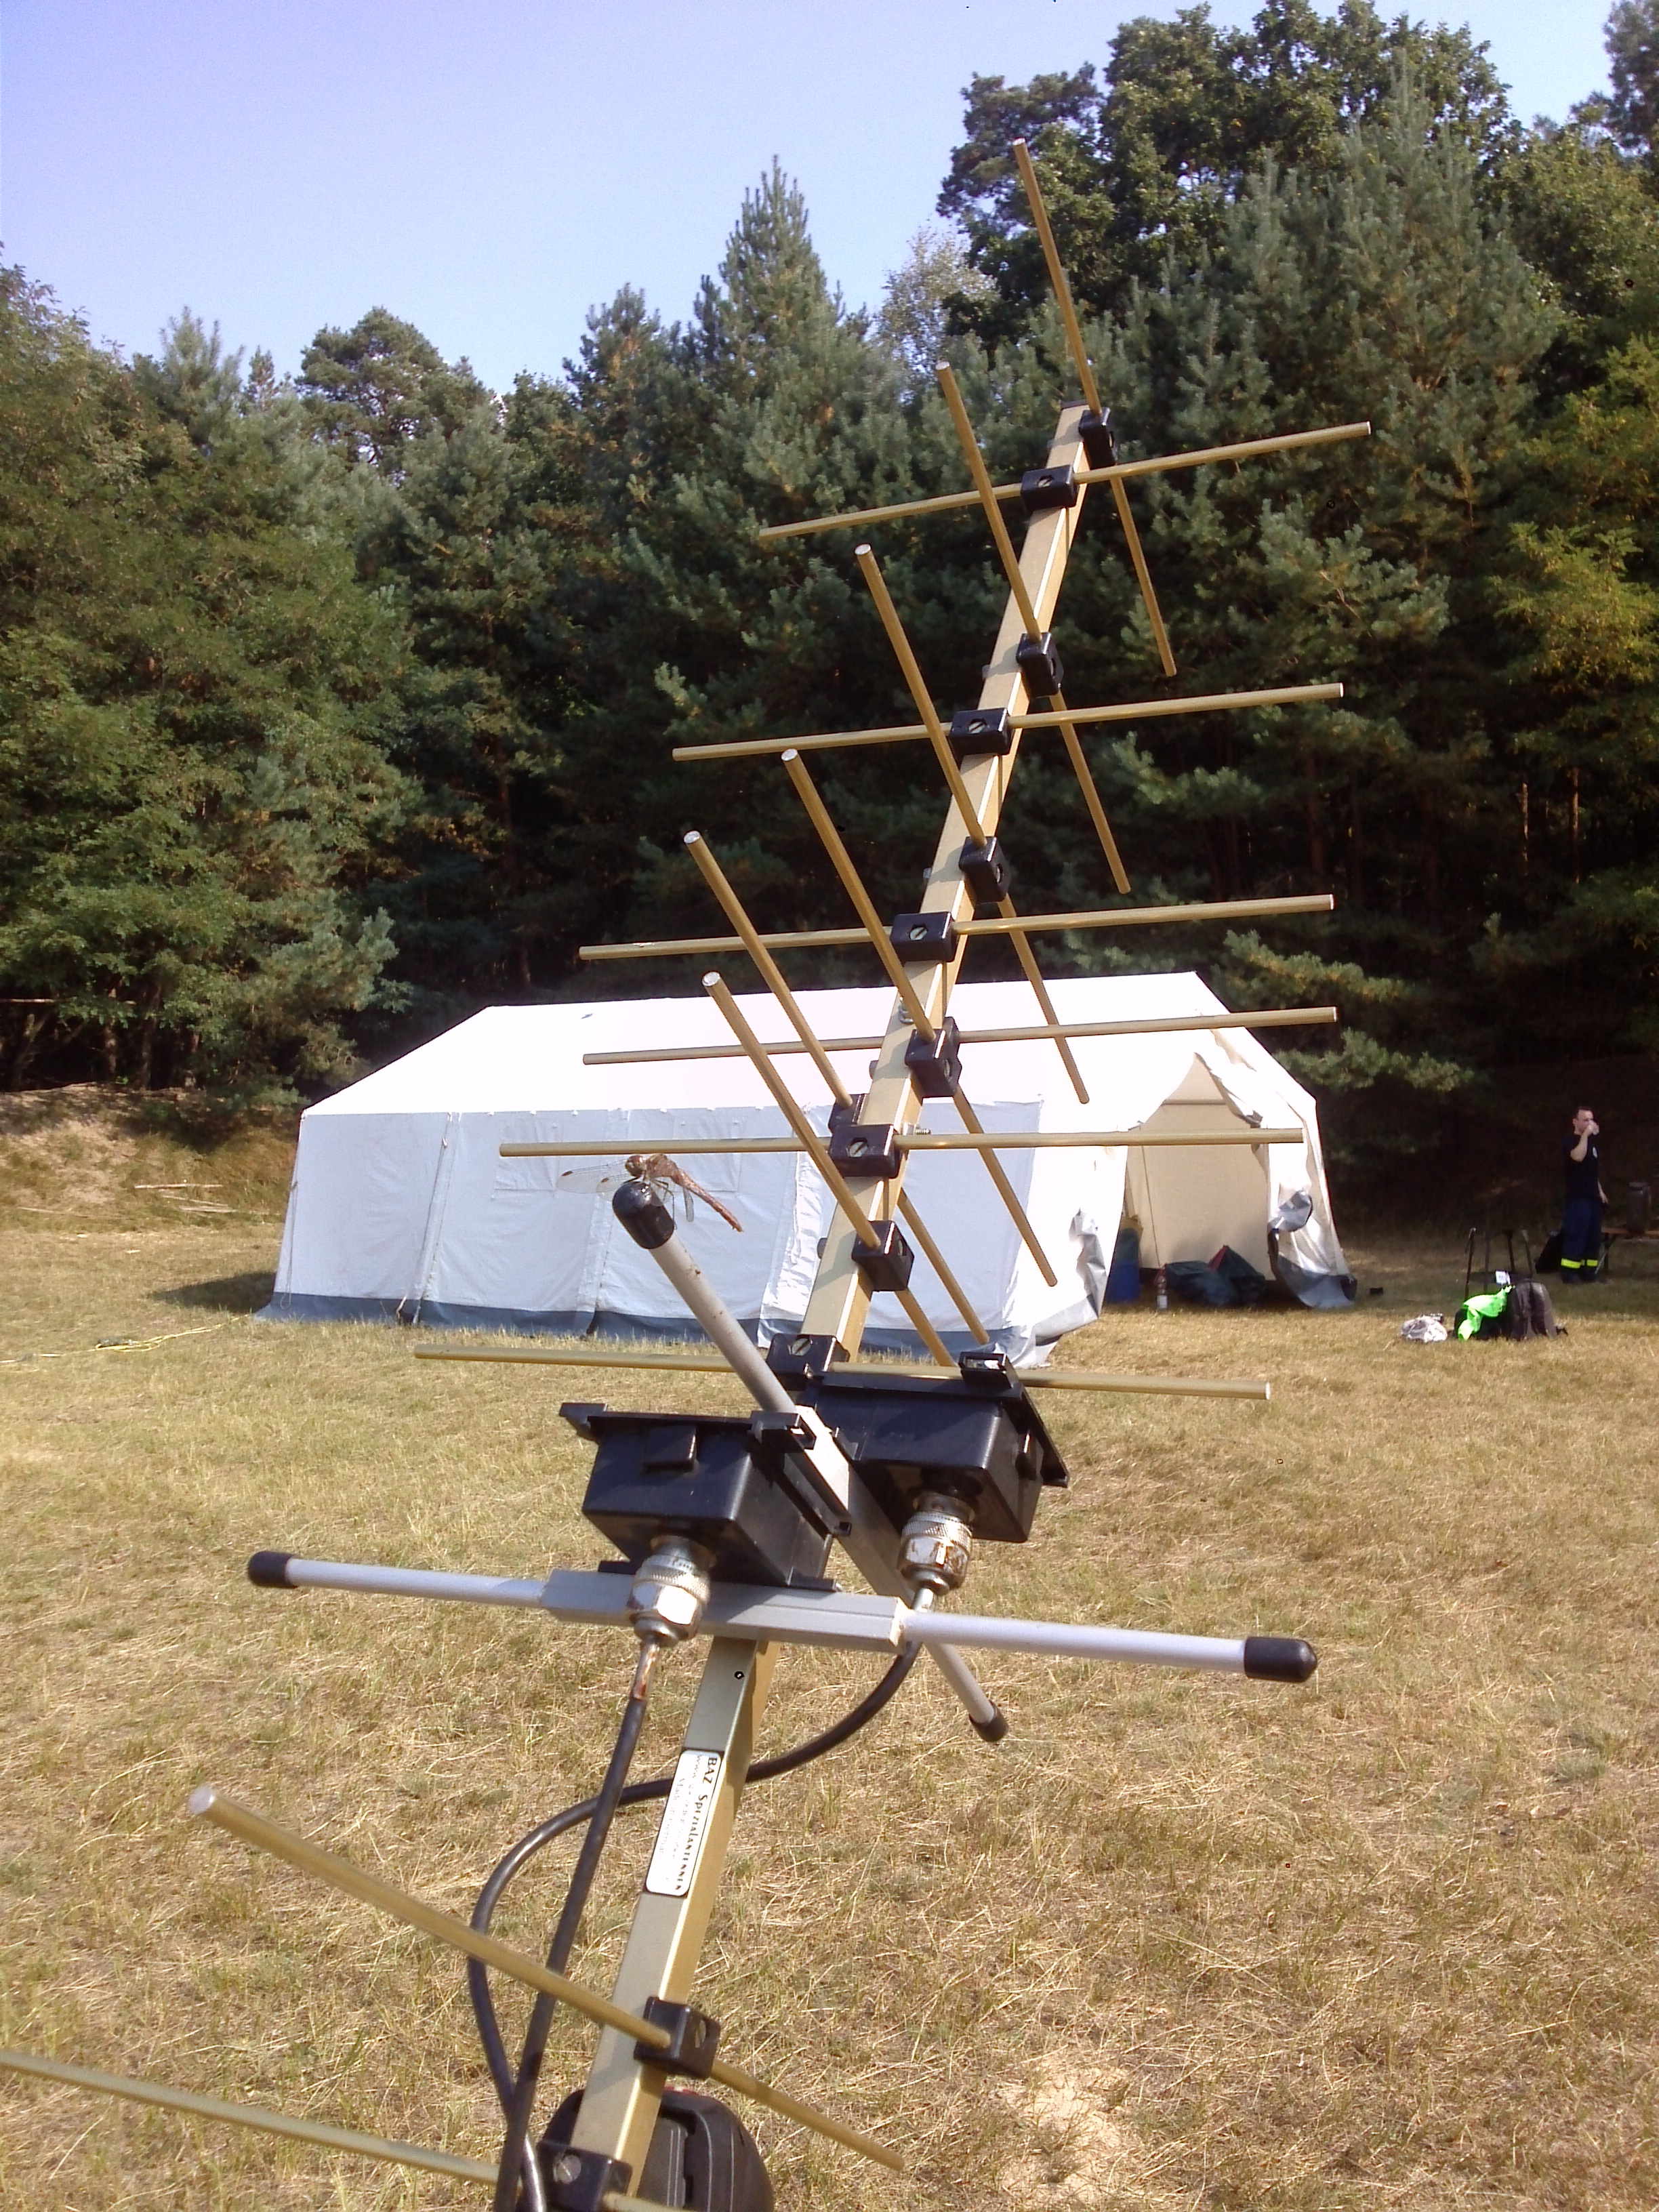
\includegraphics[width=.4\textwidth]{e11/kreutzYagi.jpg}
        \footnote{\tiny DK0TU Fildday 2014 von DL7BUR}
	\end{center}
\end{frame}

\begin{frame}
    \frametitle{Jetzt Ihr}
    \begin{center} 	Baut, messt und benutzt eure selbstgebauten Antennen
        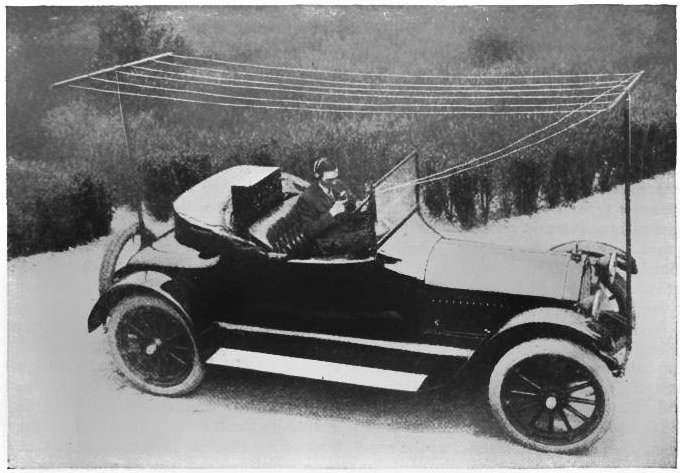
\includegraphics[width=1\textwidth]{antennen101/hamPro.jpg}
	\end{center}
\end{frame}

\begin{frame}
    \frametitle{Kontakt}
    	\begin{itemize}
		\item Twitter: [at]b4um oder [at]dk0tu
		\item baum AT campus.tu-berlin.de
		\item GSM: B4UM
		\item Amateur Radio Dorf
    \end{itemize}
\end{frame}


\section*{Referenzen}

\begin{frame}
    \frametitle{Referenzen/Links}
    
    \footnotesize
    \begin{itemize}
        \item Moltrecht E 09: \\
              \url{http://www.dj4uf.de/lehrg/e11/e11.html}
        \item Strahlungsdiagramm (Youtube): \\
              \url{https://www.youtube.com/watch?v=gBqqp7rnZ64}
    \end{itemize}

\end{frame}

% Hier könnte noch eine Kontaktfolie stehen

\end{document}


%%%%%%%%%%%%%%%%%%%%%%%%%%%%%%%%%%%%%%%%%%%%%%%%



% Foliensatz: "AFu-Kurs nach DJ4UF" von DK0TU, Amateurfunkgruppe der TU Berlin
% Lizenz: CC BY-NC-SA 3.0 de (http://creativecommons.org/licenses/by-nc-sa/3.0/de/)
% Autoren: Felix Baum <baum@campus.tu-berlin.de>

\documentclass[aspectratio=169]{beamer}

\usepackage[ngerman]{babel} % deutsche Worttrennung etc.
\usepackage[utf8]{inputenc} % UTF8 Text

\usepackage[super, comma, numbers, square, sort]{natbib}

\usepackage{hyperref}       % Hyperref Package für bessere Referenzen (todo)
\hypersetup{
	colorlinks=false,       %   false: boxed links; true: colored links
    %linkcolor=white,       %   color of internal links (change box color with linkbordercolor)
    citecolor=red,          %   color of links to bibliography
    filecolor=white,        %   color of file links
    urlcolor=blue           %   color of external links
}

\usepackage{multirow}
\usepackage{wasysym}  % Math Symbols like \permil
%\usepackage{colortbl}
%\usepackage{subscript}
%\usepackage{caption}
%\usepackage{setspace}
%\usepackage{xcolor}        % benutze CodeListe

% Footnote
%\usepackage{hanging}
%
%\setbeamertemplate{footnote}{%
%  \hangpara{2em}{1}%
%  \makebox[2em][l]{\insertfootnotemark}\footnotesize\insertfootnotetext\par%
%}


%\usepackage{pgf}
%\usepackage{tikz}
%\usetikzlibrary{arrows,automata}
%\usetikzlibrary{positioning}
%
%\tikzset{
%    state/.style={
%           rectangle,
%           rounded corners,
%           draw=black, very thick,
%           minimum height=2em,
%           minimum width=2pt,
%           inner sep=2pt,
%           text centered,
%           },
%}

%\usepackage{listings}
%\lstset{basicstyle=\small, numberstyle=\tiny, extendedchars=true, numbers=left, numbersep=5pt}
%\lstset{showtabs=false, showspaces=false, showstringspaces=false}
%%\lstset{backgroundcolor=\color{white!75!lightgray}, , frame=single}
%%\lstset{backgroundcolor=\color{white}}
%%\lstset{backgroundcolor=none}
%\lstset{keywordstyle=\color{blue!50!gray},  identifierstyle=\color{black}}
%\lstset{commentstyle=\color{green!50!gray}, stringstyle=\color{red!50!gray}}
%\lstset{language=C, fontadjust=true, tabsize=2, breaklines=true}
%\lstset{backgroundcolor=\color{white!75!lightgray}, caption=\lstname, frame=single}
%\lstset{emphstyle=\color{black}\fbox}
%
%% Keine "Listing:"-Caption
%\captionsetup{labelformat=empty,labelsep=none}
%
%% für mathematische Umgebungen
%\usepackage{amsmath,amsfonts,amssymb}
%
%\lstdefinestyle{Bash}{
%language=Bash,
%frame=single,
%rulecolor=\color{black},
%backgroundcolor=\color{gray!50},
%keywordstyle=\color{black},
%identifierstyle=,
%commentstyle=\color{black},
%stringstyle=\color{magenta!65!white},
%showstringspaces=false,
%basicstyle=\footnotesize\ttfamily\color{black},
%numbers=none,
%breaklines=true,
%captionpos=b
%}

%\usepackage{listings}
%
%\lstdefinestyle{basic}{
%    captionpos=t,%
%    basicstyle=\footnotesize\ttfamily,%
%    numberstyle=\tiny,%
%    numbers=left,%
%    stepnumber=1,%
%    frame=single,%
%    showspaces=false,%
%    showstringspaces=false,%
%    showtabs=false,%
%    %
%    keywordstyle=\color{blue},%
%    identifierstyle=,%
%    commentstyle=\color{gray},%
%    stringstyle=\color{magenta}%
%}



% fließende Boxen haben keinen Abstand
%\fboxsep0mm

% inkludiere Creative Commons Helper
%%%%%%%%%%%%%%%%%%%%%%%%%%%%%%%%%%%%%%%%%%%%%%%%%%%%%%%%%%%%%%%%
%% ccBeamer 0.1, 2007-07-02                                   %%
%% Written by Sebastian Pipping <webmaster@hartwork.org>      %%
%% ---------------------------------------------------------- %%
%% Licensed under Creative Commons Attribution-ShareAlike 3.0 %%
%% http://creativecommons.org/licenses/by-sa/3.0/             %%
%%%%%%%%%%%%%%%%%%%%%%%%%%%%%%%%%%%%%%%%%%%%%%%%%%%%%%%%%%%%%%%%


%% Images
\newcommand{\CcImageBy}[1]{%
	
\includegraphics[scale=#1]{texdata/creative_commons/cc_by_30.pdf}%
}
\newcommand{\CcImageCc}[1]{%
	
\includegraphics[scale=#1]{texdata/creative_commons/cc_cc_30.pdf}%
}
\newcommand{\CcImageDevNations}[1]{%
	
\includegraphics[scale=#1]{texdata/creative_commons/cc_dev_nations_30.pdf}%
}
\newcommand{\CcImageNc}[1]{%
	
\includegraphics[scale=#1]{texdata/creative_commons/cc_nc_30.pdf}%
}
\newcommand{\CcImageNd}[1]{%
	
\includegraphics[scale=#1]{texdata/creative_commons/cc_nd_30.pdf}%
}
\newcommand{\CcImagePd}[1]{%
	
\includegraphics[scale=#1]{texdata/creative_commons/cc_pd_30.pdf}%
}
\newcommand{\CcImageSa}[1]{%
	
\includegraphics[scale=#1]{texdata/creative_commons/cc_sa_30.pdf}%
}
\newcommand{\CcImageSampling}[1]{%
	
\includegraphics[scale=#1]{texdata/creative_commons/cc_sampling_30.pdf}%
}
\newcommand{\CcImageSamplingPlus}[1]{%
	
\includegraphics[scale=#1]{texdata/creative_commons/cc_sampling_plus_30.pdf}%
}


%% Groups
\newcommand{\CcGroupBy}[2]{% zoom, gap
	\CcImageCc{#1}\hspace*{#2}\CcImageBy{#1}%
}
\newcommand{\CcGroupByNc}[2]{% zoom, gap
	\CcImageCc{#1}\hspace*{#2}\CcImageBy{#1}\hspace*{#2}\CcImageNc{#1}%
}
\newcommand{\CcGroupByNcNd}[2]{% zoom, gap
	\CcImageCc{#1}\hspace*{#2}\CcImageBy{#1}\hspace*{#2}\CcImageNc{#1}\hspace*{#2}\CcImageNd{#1}%
}
\newcommand{\CcGroupByNcSa}[2]{% zoom, gap
	\CcImageCc{#1}\hspace*{#2}\CcImageBy{#1}\hspace*{#2}\CcImageNc{#1}\hspace*{#2}\CcImageSa{#1}%
}
\newcommand{\CcGroupByNd}[2]{% zoom, gap
	\CcImageCc{#1}\hspace*{#2}\CcImageBy{#1}\hspace*{#2}\CcImageNd{#1}%
}
\newcommand{\CcGroupBySa}[2]{% zoom, gap
	\CcImageCc{#1}\hspace*{#2}\CcImageBy{#1}\hspace*{#2}\CcImageSa{#1}%
}
\newcommand{\CcGroupDevNations}[2]{% zoom, gap
	\CcImageCc{#1}\hspace*{#2}\CcImageDevNations{#1}%
}
\newcommand{\CcGroupNcSampling}[2]{% zoom, gap
	\CcImageCc{#1}\hspace*{#2}\CcImageNc{#1}\hspace*{#2}\CcImageSampling{#1}%
}
\newcommand{\CcGroupPd}[1]{% zoom
	\CcImagePd{#1}%
}
\newcommand{\CcGroupSampling}[1]{% zoom
	\CcImageSampling{#1}%
}
\newcommand{\CcGroupSamplingPlus}[1]{% zoom
	\CcImageSamplingPlus{#1}%
}


%% Text
\newcommand{\CcLongnameBy}{Attribution}
\newcommand{\CcLongnameByNc}{Attribution-NonCommercial}
\newcommand{\CcLongnameByNcNd}{Attribution-NoDerivs}
\newcommand{\CcLongnameByNcSa}{Attribution-NonCommercial-ShareAlike}
\newcommand{\CcLongnameByNd}{Attribution-NoDerivs}
\newcommand{\CcLongnameBySa}{Attribution-ShareAlike}

\newcommand{\CcNote}[1]{% longname
	This work is licensed under the \textit{Creative Commons #1 3.0 License}.%
}


% generelles Thema auswählen
\usetheme{Goettingen} %Berlin spart ohne Sidebar allerdings angenehm Platz
% AnnArbor | Antibes | Bergen | Berkeley | Berlin | Boadilla | boxes | CambridgeUS | Copenhagen | Darmstadt | default | Dresden | Frankfurt | Goettingen | Hannover | Ilmenau | JuanLesPins | Luebeck | Madrid | Malmoe | Marburg | Montpellier | PaloAlto | Pittsburgh | Rochester | Singapore | Szeged | Warsaw

% Farben wählen
\usecolortheme{beetle}
% beaver | beetle | crane | default | dolphin | dove | fly | lily | orchid | rose | seagull | seahorse | sidebartab | structure | whale | wolverine

% Setze alle Farben auf Grau und Weiß
%\definecolor{craneorange}{RGB}{64,64,64}
%\definecolor{craneblue}{RGB}{255,255,255}

% Schriftart wählen
\usefonttheme{default}
% default | professionalfonts | serif | structurebold | structureitalicserif | structuresmallcapsserif

% Innere Themen(Kopf-, Fuß-, Sidebar usw)
%\useinnertheme{default}
\useinnertheme{circles}
% default | inmargin | rectangles | rounded | circles

% Äußere Themen (Anordnung der inneren, grenzen der Folien etc.)
\useoutertheme{infolines}
% default | infolines | miniframes | shadow | sidebar | smoothbars | smoothtree | split | tree

% Deaktiviere Navigations-Symbole ({} -> leer)
\setbeamertemplate{navigation symbols}{}
%\setbeamertemplate{navigation symbols}{\large \ifnum \insertframenumber <10 0\fi\insertframenumber/\inserttotalframenumber\vspace*{0.2ex}}

% Zeige ein Hintergrundbild
\setbeamertemplate{background canvas}{
        \hspace*{-2.0cm}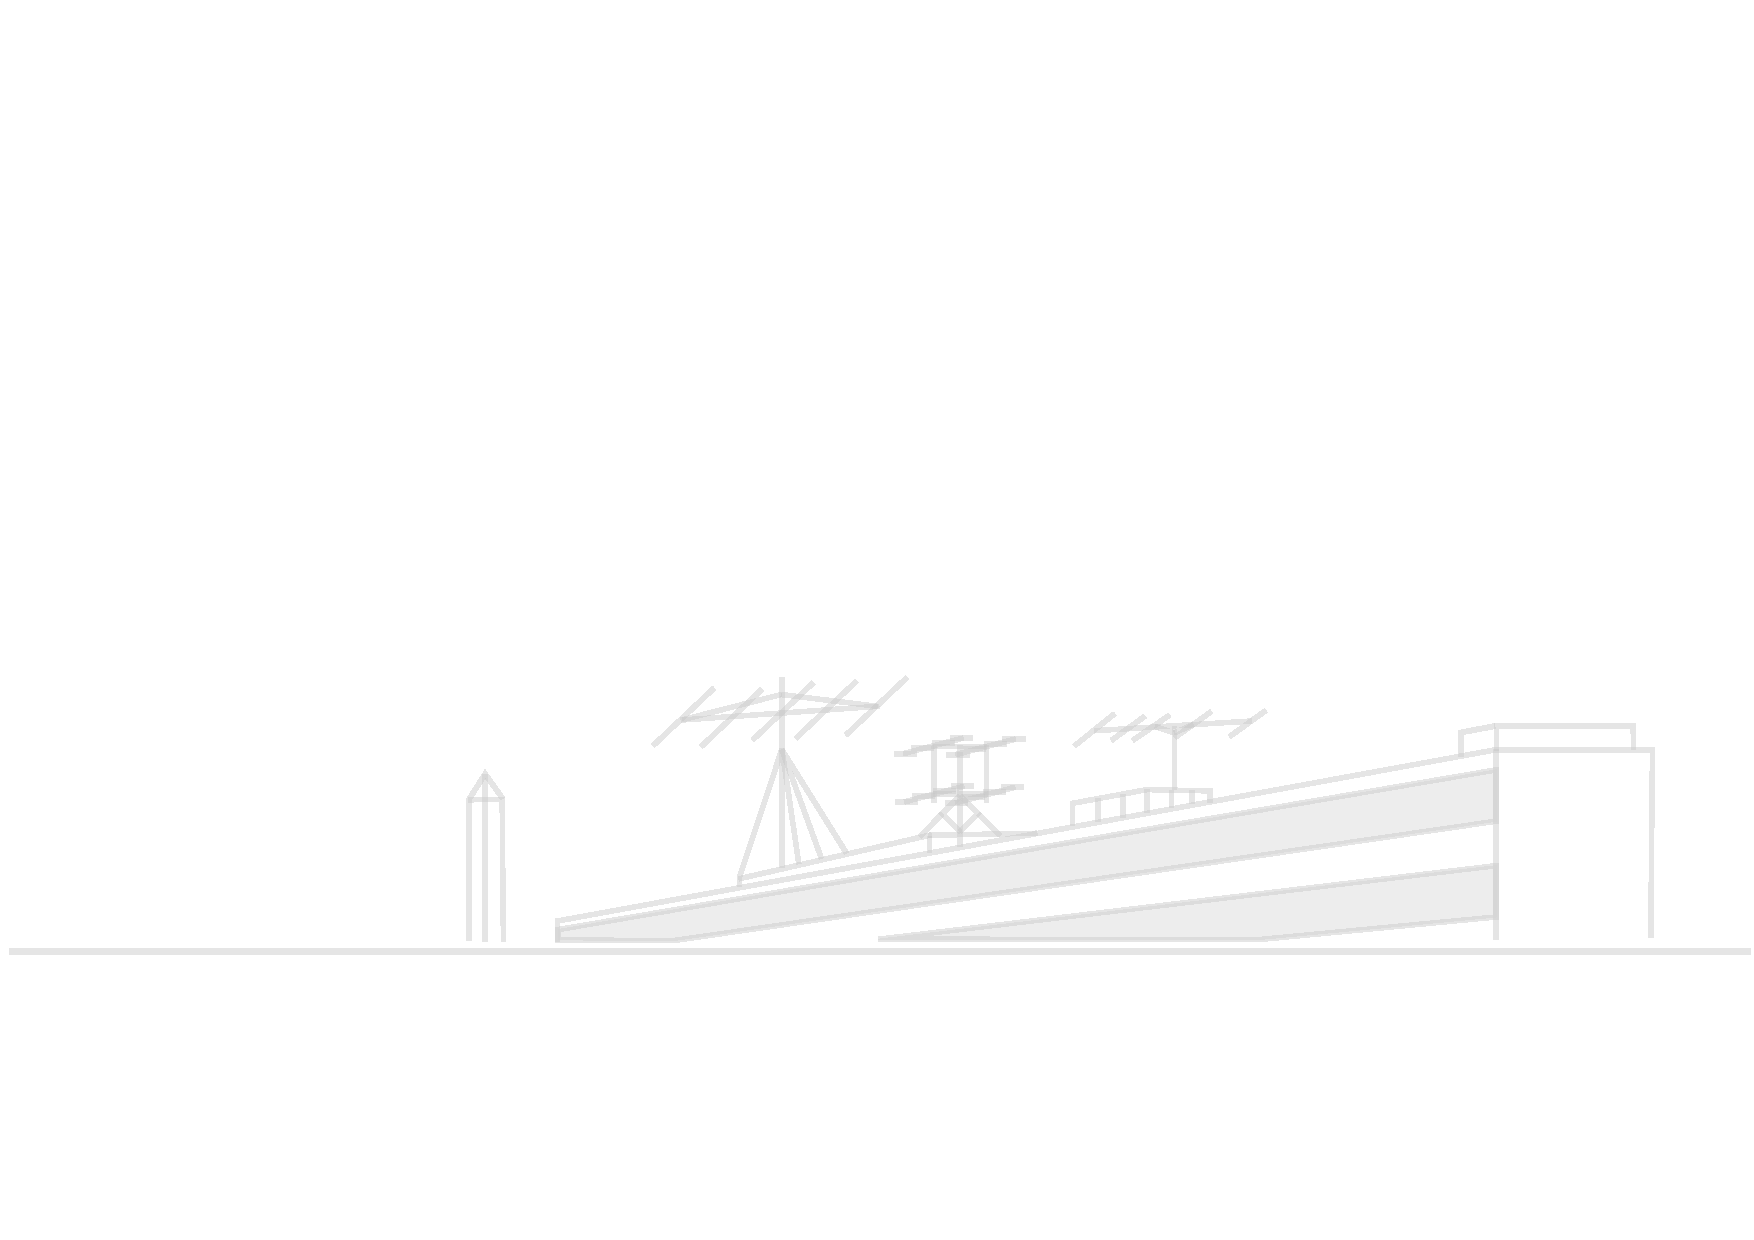
\includegraphics[width=17.8cm]{texdata/dk0tu_rooftop_background.pdf}
}

% Foliennummer einfügen
\setbeamertemplate{footline}[frame number]
%\setbeamertemplate{footline}{}

% Ändere das Zeichen vor jedem item
%\setbeamertemplate{itemize item}{\color{craneorange}$\blacktriangleright$}
%\setbeamertemplate{itemize subitem}{\color{craneorange}$\triangleright$}
%\setbeamertemplate{itemize subsubitem}{\color{craneorange}$\blacktriangleright$}

% Ändert die Blöcke 
\setbeamertemplate{blocks}[rounded][shadow=true]
% default | rounded [shadow=true|false]

%
% Eigene Kommandos
%

% Hack to get natbib and beamer working together. "The beamer user guide suggests
% that only the manual bibliography entry approach is supported"
% on some system it works out of the box, sometimes you need the hack :-(
% so check it --dl7bst
\ifdefined\newblock
    \relax
\else
    \newcommand{\newblock}{}
\fi

% \includedia command to generate png out of a dia file
% NEEDS installed dia and pdflatex option --shell-escape
\newcommand{\includedia}[1]{
    \immediate\write18{/usr/bin/dia #1.dia -e #1_diatmp.png -t png}
}

% RICHIG GROSSER FONT!
\newfont{\bigfont}{cmr10 at 144pt}
\newfont{\smallfont}{cmr10 at 8pt}

% Römische Ziffern
\makeatletter
\newcommand{\rmnum}[1]{\romannumeral #1}
\newcommand{\Rmnum}[1]{\expandafter\@slowromancap\romannumeral #1@}
\makeatother

% Schwarze Überschrift
%\setbeamercolor{frametitle}{fg=black}
%\setbeamercolor{title}{fg=black}

% Item- und Box-Farben
\definecolor{deepBlue}{HTML}{000066}
\setbeamercolor{itemize item}{fg=deepBlue}
\setbeamercolor{itemize subitem}{fg=deepBlue}
\setbeamercolor{description item}{fg=deepBlue}
\setbeamercolor{block title}{fg=deepBlue!100, bg=blue!15}
\setbeamercolor{block body}{fg=black, bg=blue!5}
\setbeamercolor{block title alerted}{fg=deepBlue, bg=red!75}
\setbeamercolor{block body alerted}{fg=black, bg=red!15}
\setbeamercolor*{block title example}{fg=blue!50, bg=blue!10}
\setbeamercolor*{block body example}{fg= blue, bg=blue!5}

%\setbeamercolor{section in head/foot}{parent=palette primary}
%\setbeamercolor{subsection in head/foot}{parent=palette secondary}
%\setbeamercolor{sidebar}{fg=darkblue,bg=yellow!90!orange}
%\setbeamercolor{title in sidebar}{fg=darkblue}
%\setbeamercolor{author in sidebar}{fg=darkblue}
%\setbeamercolor{section in sidebar}{fg=darkblue!10!black}
%\setbeamercolor{subsection in sidebar}{fg=darkblue!50!black}

% Titlepage Infos
\title{AFu-Kurs nach DJ4UF}
\author[DKØTU]{DKØTU\\ \footnotesize{Amateurfunkgruppe der TU Berlin}}
\institute[DKØTU]{\url{http://www.dk0tu.de} }

% PDF-Eigenschaften
\subject{DK0TU-Amateurfunkkurs nach DJ4UF}
\keywords{Amateurfunk Kurs HAM Radio Course CC-BY-NC-SA OpenSource TU Berlin DK0TU}

\subtitle{Technik 11: \\
           Antennentechnik \\[2em]}
\date{Stand 30.11.2014}
 \begin{document}

\begin{frame}
    \titlepage
    \vfill
    \begin{center}
        \ccbyncsaeu\\
        {\tiny This work is licensed under the \em{Creative Commons Attribution-NonCommercial-ShareAlike 3.0 License}.}\\[0.5ex]
         \tiny Amateurfunkgruppe der Technische Universität Berlin (AfuTUB), DKØTU
         %\includegraphics[scale=0.5]{img/DK0TU_Logo.pdf}
    \end{center}
\end{frame}


%fixme Referenzen/Fußnoten-Systematik vereinheitlichen

\section*{Einleitung}

\begin{frame}
    \frametitle{Antenne}
      \begin{center}
        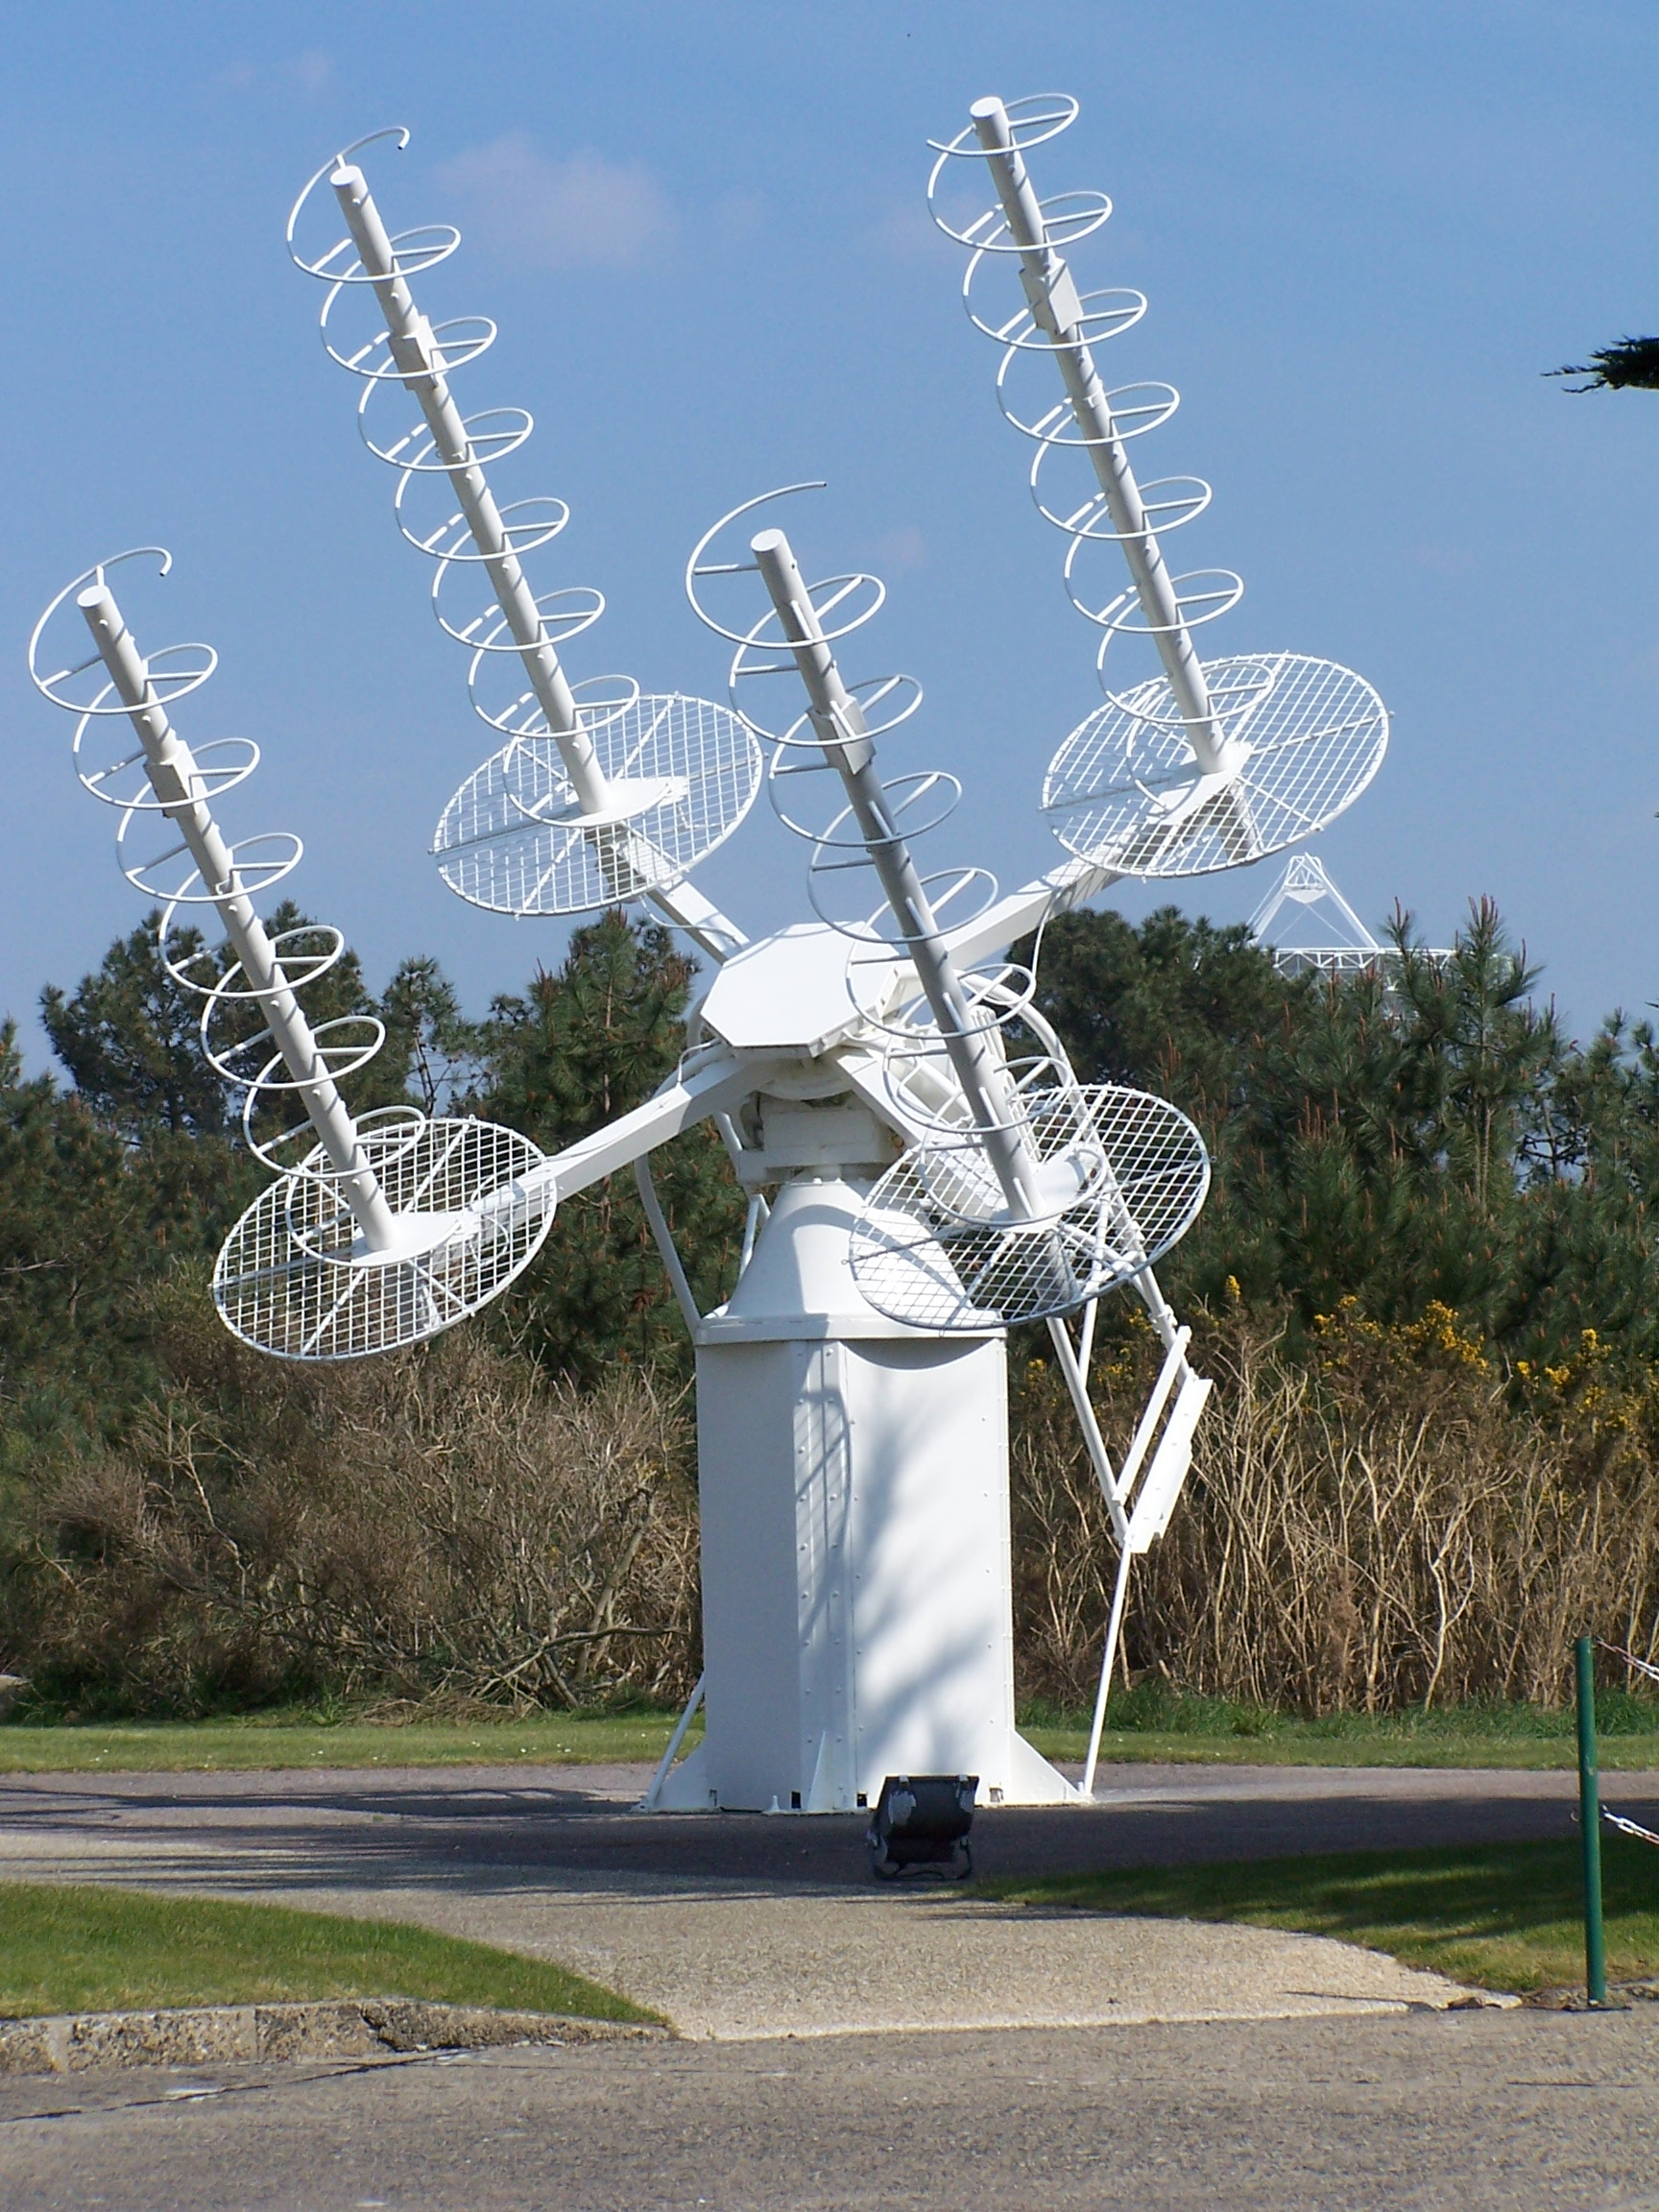
\includegraphics[width=.5\textwidth]{e11/Traqueur_acquisition.JPG}
        \footnote{\tiny \url{https://upload.wikimedia.org/wikipedia/commons/3/32/Traqueur_acquisition.JPG}}
    \end{center}
\end{frame}
  

\begin{frame}
    \frametitle{Allgemeines}
	\begin{itemize}
		\item Jeder ungeschirmte Draht ist eine Antenne
        \item Grundsätzlich sind Sende und Emfangsantennen ähnlich
        \item Alle guten KW Sendeantennen sind auch gute Emfangsantennen
       	\item Umgekehrt nicht immer der Fall (z.B. Ferritantenne)
    \end{itemize}
\end{frame}

\begin{frame}
    \frametitle{Vorstellung}
    \begin{center}
        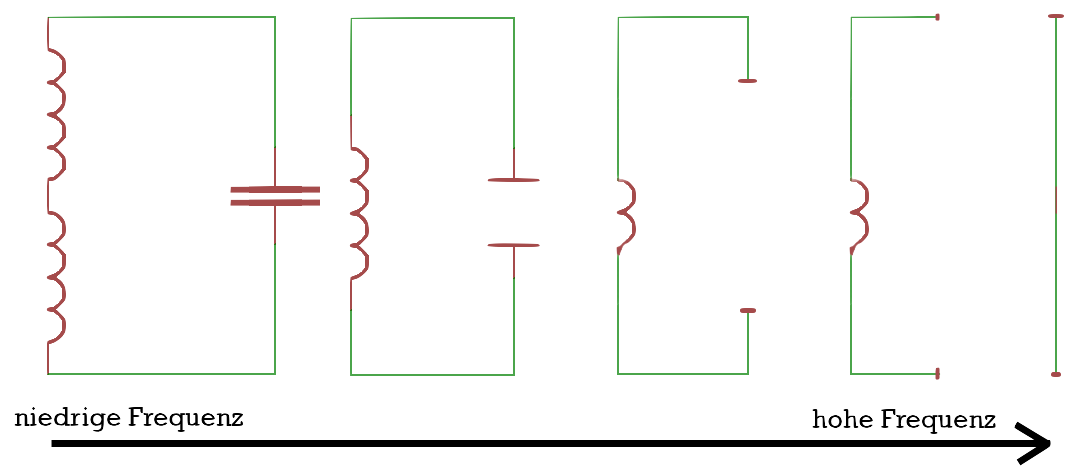
\includegraphics[width=1\textwidth]{e11/dipol_entstehung.png}
        \footnote{\tiny by DB4UM}
	\end{center}
\end{frame}

\begin{frame}
    \frametitle{E- und H-Feld}
    \begin{center}
        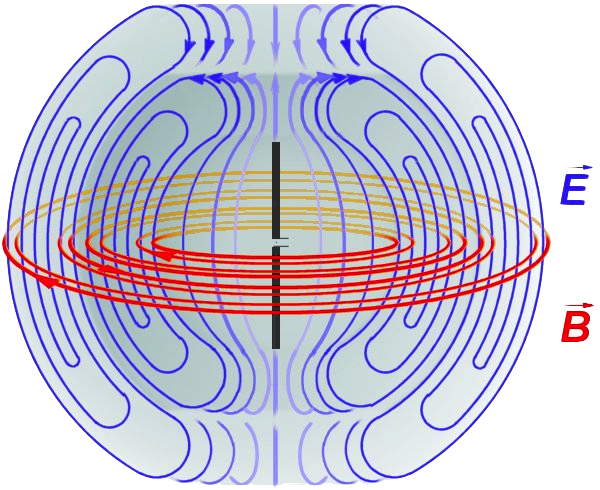
\includegraphics[width=0.85\textwidth]{e11/Felder_um_Dipol.png}
        \footnote{\tiny \url{https://commons.wikimedia.org/wiki/File:Felder_um_Dipol.jpg}}
	\end{center}
\end{frame}


\section*{Dipol}

\begin{frame}
    \frametitle{Strom und Spannungsverteilung}
	\begin{itemize}
		\item Stahlerlänge $\lambda / 2$
		\item Stromknoten und Spannungsbauch an den Enden (Unendlich großer Widerstand)
        \item Spannungsknoten und Strombauch in der Mitte (fast $0 \Omega$ Widerstand)
    \end{itemize}
    \begin{center}
        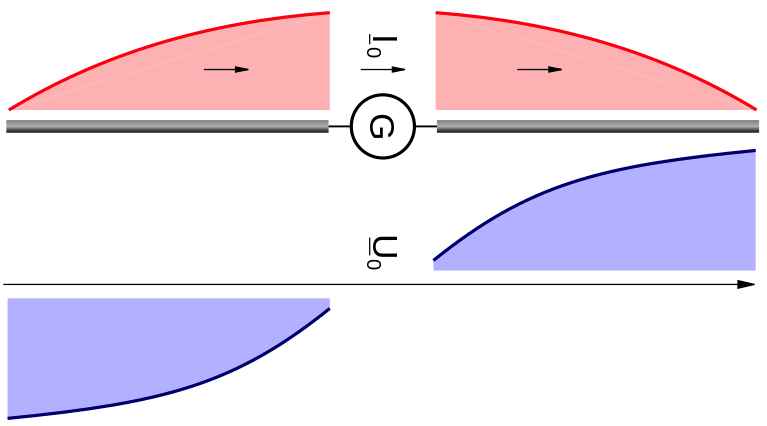
\includegraphics[width=0.85\textwidth]{e11/DipolUI.png}
        \footnote{\tiny \url{https://commons.wikimedia.org/wiki/File:Lineare_antennen.svg}}
	\end{center}
\end{frame}

\begin{frame}
    \frametitle{Fußpunktwiderstand}
    \begin{center}
	\begin{itemize}
		\item Fußpunktwiderstand/Impedanz/Speisewiderstand
		\item Beim Dipol im Freien Raum: $70 \Omega$
		\item je nach Dipolhöhe zwischen $40  \Omega$ und $80  \Omega$
		\item  Bei $0.15 \lambda$ Höhe $50  \Omega$ Speisewiderstand 
    \end{itemize}
 	\end{center}
\end{frame}

\begin{frame}
    \frametitle{Prüfungsfrage}

    \begin{center}
    \begin{tabular}{l||l}\hline
        TH206 & Ein Halbwellendipol wird auf der  \\
         " "  & Grundfrequenz in der Mitte \\ \hline\hline
         A & spannungsgespeist.\\\hline
         B & stromgespeist. \\\hline
         C & endgespeist. \\ \hline
         D & parallel gespeist.\\\hline
    \end{tabular}
 	\end{center}
\end{frame}

\begin{frame}
    \frametitle{Prüfungsfrage}

    \begin{center}
    \begin{tabular}{l||l}\hline
        TH206 & Ein Halbwellendipol wird auf der  \\
         " "  & Grundfrequenz in der Mitte \\ \hline\hline
         " " & spannungsgespeist.\\\hline
         X & stromgespeist. \\\hline
         " " & endgespeist. \\ \hline
         " " & parallel gespeist.\\\hline
    \end{tabular}
        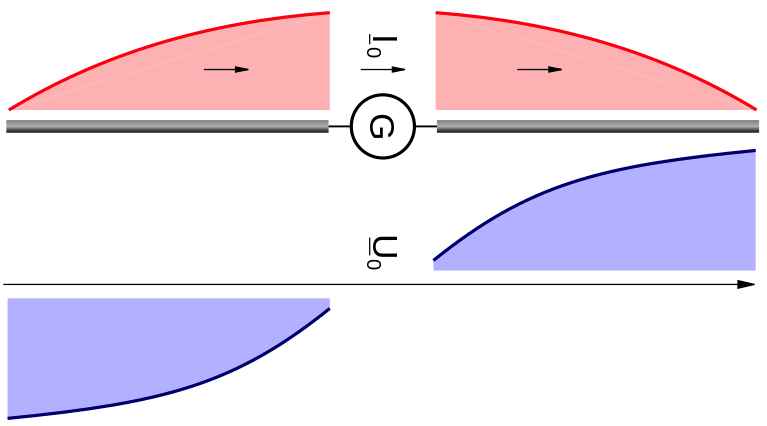
\includegraphics[width=0.85\textwidth]{e11/DipolUI.png}
        \footnote{\tiny \url{https://commons.wikimedia.org/wiki/File:Lineare_antennen.svg}}
 	\end{center}
\end{frame}
    
\begin{frame}
    \frametitle{$\lambda / 2$ Dipol berechnen}
    \begin{center}
	\begin{itemize}
		\item Aufgabe:
		\item Theoretische Strahlerlänge eines $\lambda / 2$ Dipols für 7MHz berechnen
		\item Warum in der Praxis Verkürzungsfaktor?
    \end{itemize}
        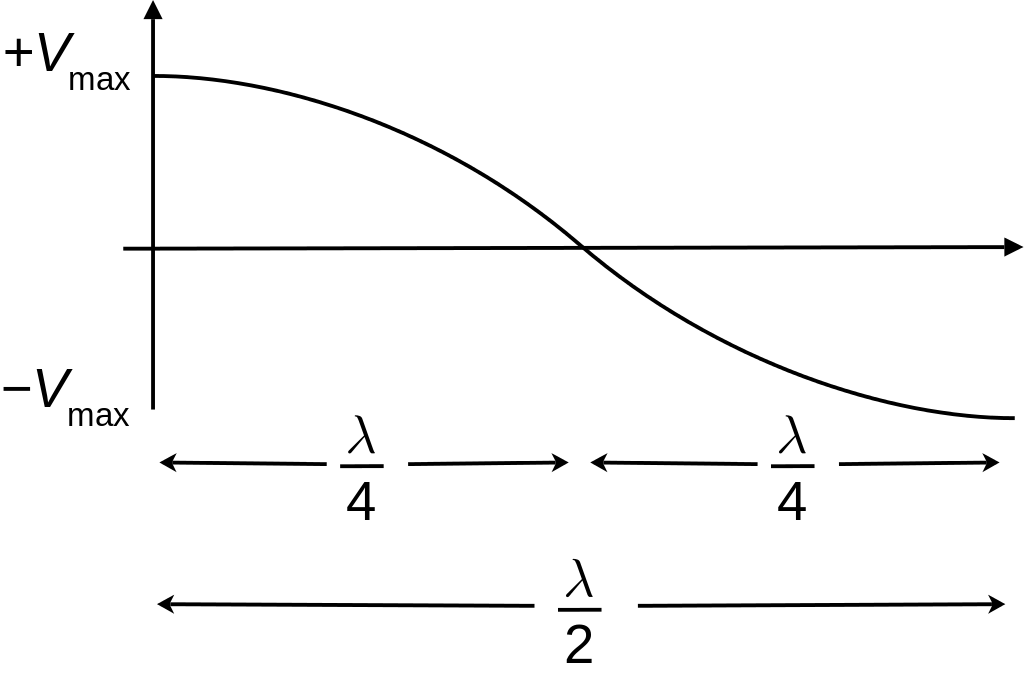
\includegraphics[width=0.75\textwidth]{e11/Dipole_Antenna.png}
        \footnote{\tiny \url{https://commons.wikimedia.org/wiki/File:Dipole_Antenna.svg}}
 	\end{center}
\end{frame}

\section*{Richtdiagramm}

\begin{frame}
    \frametitle{Richtdiagramm Dipol}
    \begin{center}
        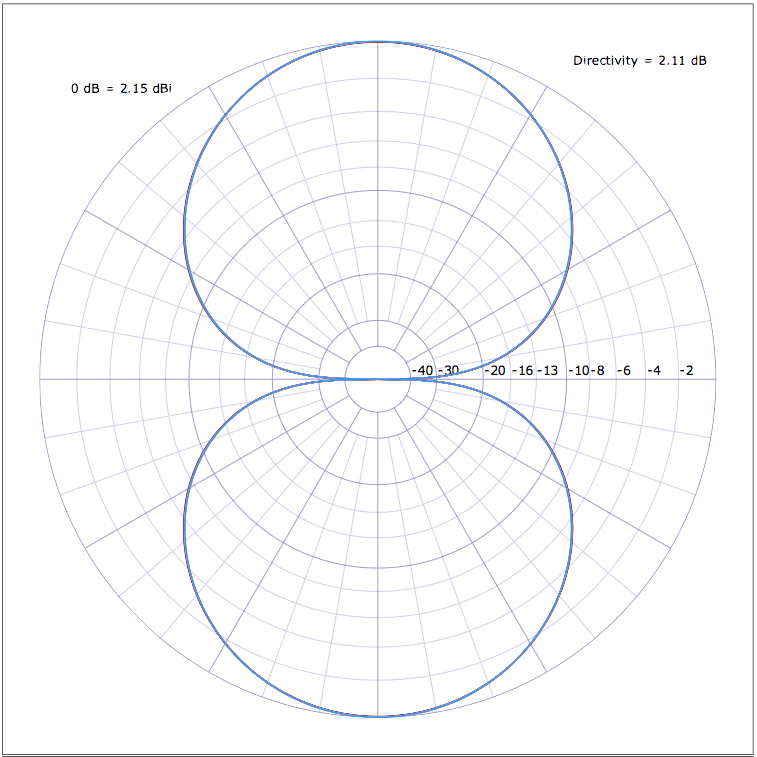
\includegraphics[width=0.75\textwidth]{e11/Richt-Dipol.png}
        \footnote{\tiny DB4UM Programm: cocoaNec 2.0}
	\end{center}
\end{frame}

\begin{frame}
    \frametitle{Richtdiagramm Yagi}
    \begin{center}
        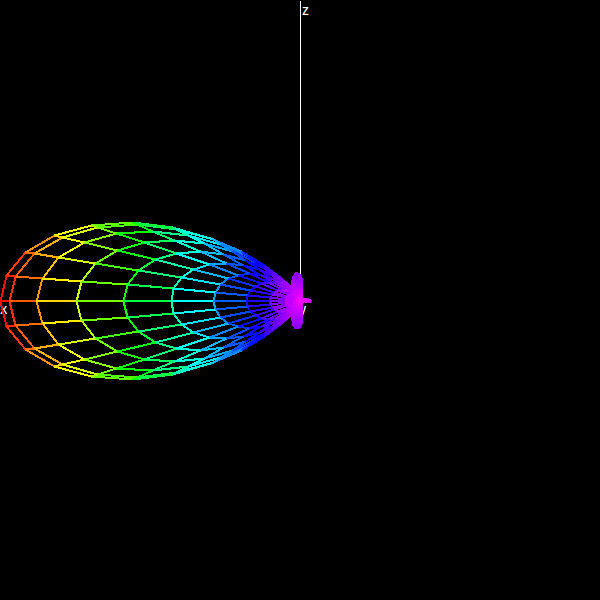
\includegraphics[width=0.75\textwidth]{e11/yagi_gain.png}
        \footnote{\tiny DK0TU 10m Yagi 28.2 MHz von DL2JAS Programm: EZNEC}
	\end{center}
\end{frame}

\section*{Gewinn}

\begin{frame}
    \frametitle{EIRP und ERP}
    \begin{itemize}
    	\item ERP
		    \begin{itemize}
				\item Effektive Radiated Power
       		 	\item Bezug auf Dipol
       		 	\item $P_{ERP} = G_{Dipol} \cdot (P_{Sender} - P_{Verlust})$
 		   	\end{itemize}
		\item EIRP
		    \begin{itemize}
				\item Effektive Isotropic Radiated Power
       		 	\item Bezug auf Isotropstrahler
       		 	\item $dB_{ERP} = 2.15 + dB_{EIRP}$
       		 	\item $P_{EIRP} = 1.64 \cdot P_{ERP}$
 		   	\end{itemize}
    \end{itemize}
\end{frame}

\begin{frame}
    \frametitle{Isotropstrahler}
    \begin{center}
        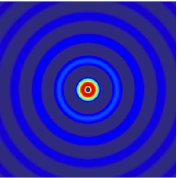
\includegraphics[width=0.75\textwidth]{e11/Spherical_wave2.png}
        \footnote{\tiny \url{https://commons.wikimedia.org/wiki/File:Spherical_wave2.gif}}
	\end{center}
\end{frame}

\begin{frame}
    \frametitle{Prüfungsfrage}

    \begin{center}
    \begin{tabular}{l||l}\hline
        TL205 & Ein Sender mit 5 Watt Ausgangsleistung ist über\\
        " "  & eine Antennenleitung, die 2 dB Kabelverluste hat,\\
        " "  & an eine Antenne mit 5 dB Gewinn (auf Dipol\\
        " "  & bezogen) angeschlossen. Welche EIRP wird von \\
        " "  &  der Antenne maximal abgestrahlt?\\\hline\hline
         A 	  & 32,8 Watt \\\hline
         B 	  & 10,0 Watt \\\hline
         C	  & 6,1 Watt \\\hline
         D 	  & 16,4 Watt\\\hline
    \end{tabular}
 	\end{center}
\end{frame}

\begin{frame}
    \frametitle{Prüfungsfrage}

    \begin{center}
    \begin{tabular}{l||l}\hline
        TL205 & Ein Sender mit 5 Watt Ausgangsleistung ist über\\
        " "  & eine Antennenleitung, die 2 dB Kabelverluste hat,\\
        " "  & an eine Antenne mit 5 dB Gewinn (auf Dipol\\
        " "  & bezogen) angeschlossen. Welche EIRP wird von \\
        " "  &  der Antenne maximal abgestrahlt?\\\hline\hline
         " " 	  & 32,8 Watt \\\hline
         " " 	  & 10,0 Watt \\\hline
         " "	  & 6,1 Watt \\\hline
         X 	  & 16,4 Watt\\\hline
    \end{tabular}
 	\end{center}
\end{frame}

\section*{Multiband}

\begin{frame}
    \frametitle{Multiband Dipol}
    \begin{center}
        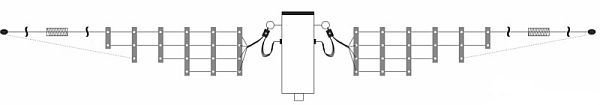
\includegraphics[width=0.9\textwidth]{e11/Multiband.jpg}
        \footnote{\tiny Antenne EA-1015204080 von EAntenna}
	\end{center}
\end{frame}

\begin{frame}
    \frametitle{G5RV}
    \begin{center}
        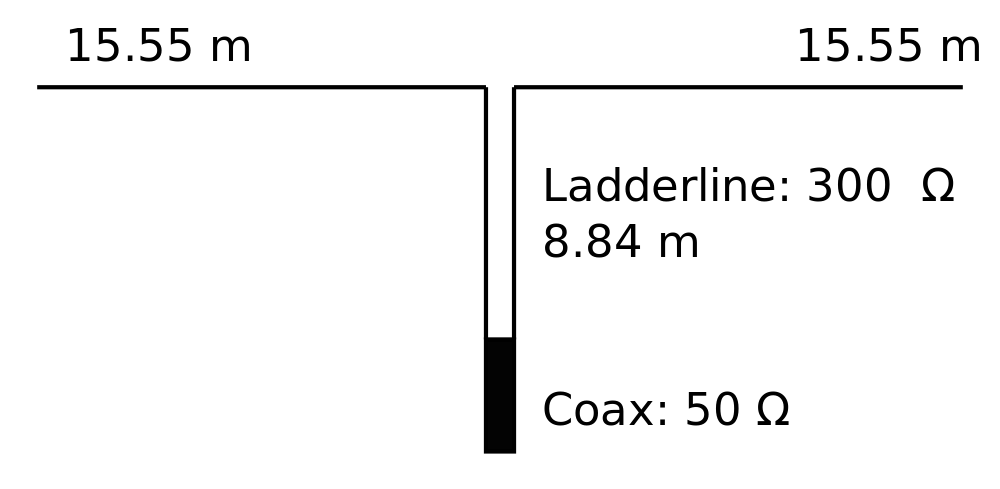
\includegraphics[width=0.9\textwidth]{e11/G5RV_Antenna.png}
        \footnote{\tiny \url{https://commons.wikimedia.org/wiki/File:G5RV_Antenna.svg}}
	\end{center}
\end{frame}

\section*{Endgespeist}

\begin{frame}
    \frametitle{Fuchskreis}
    \begin{center}
        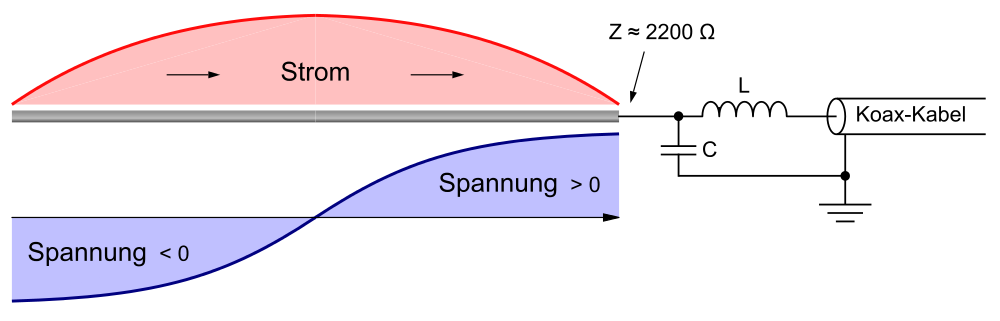
\includegraphics[width=1\textwidth]{e11/1000px-Endgespeiste_Antenne.png}
        \footnote{\tiny \url{https://commons.wikimedia.org/wiki/File:Endgespeiste_Antenne.svg}}
	\end{center}
\end{frame}

\section*{Yagi-Uda}

\begin{frame}
    \frametitle{Yagi-Uda}
    \begin{center}
        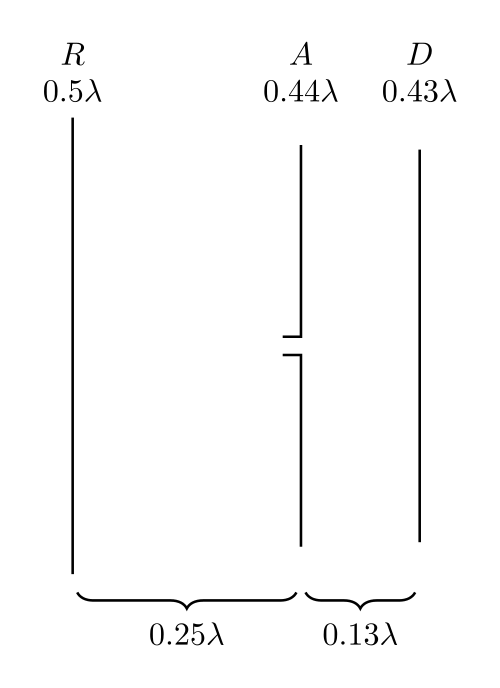
\includegraphics[width=0.5\textwidth]{e11/Yagi_3_element.png}
        \footnote{\tiny \url{https://commons.wikimedia.org/wiki/File:Yagi_3_element.svg}}
	\end{center}
\end{frame}

\begin{frame}
    \frametitle{Yagi - Richtung erkennen}
    \begin{center}
        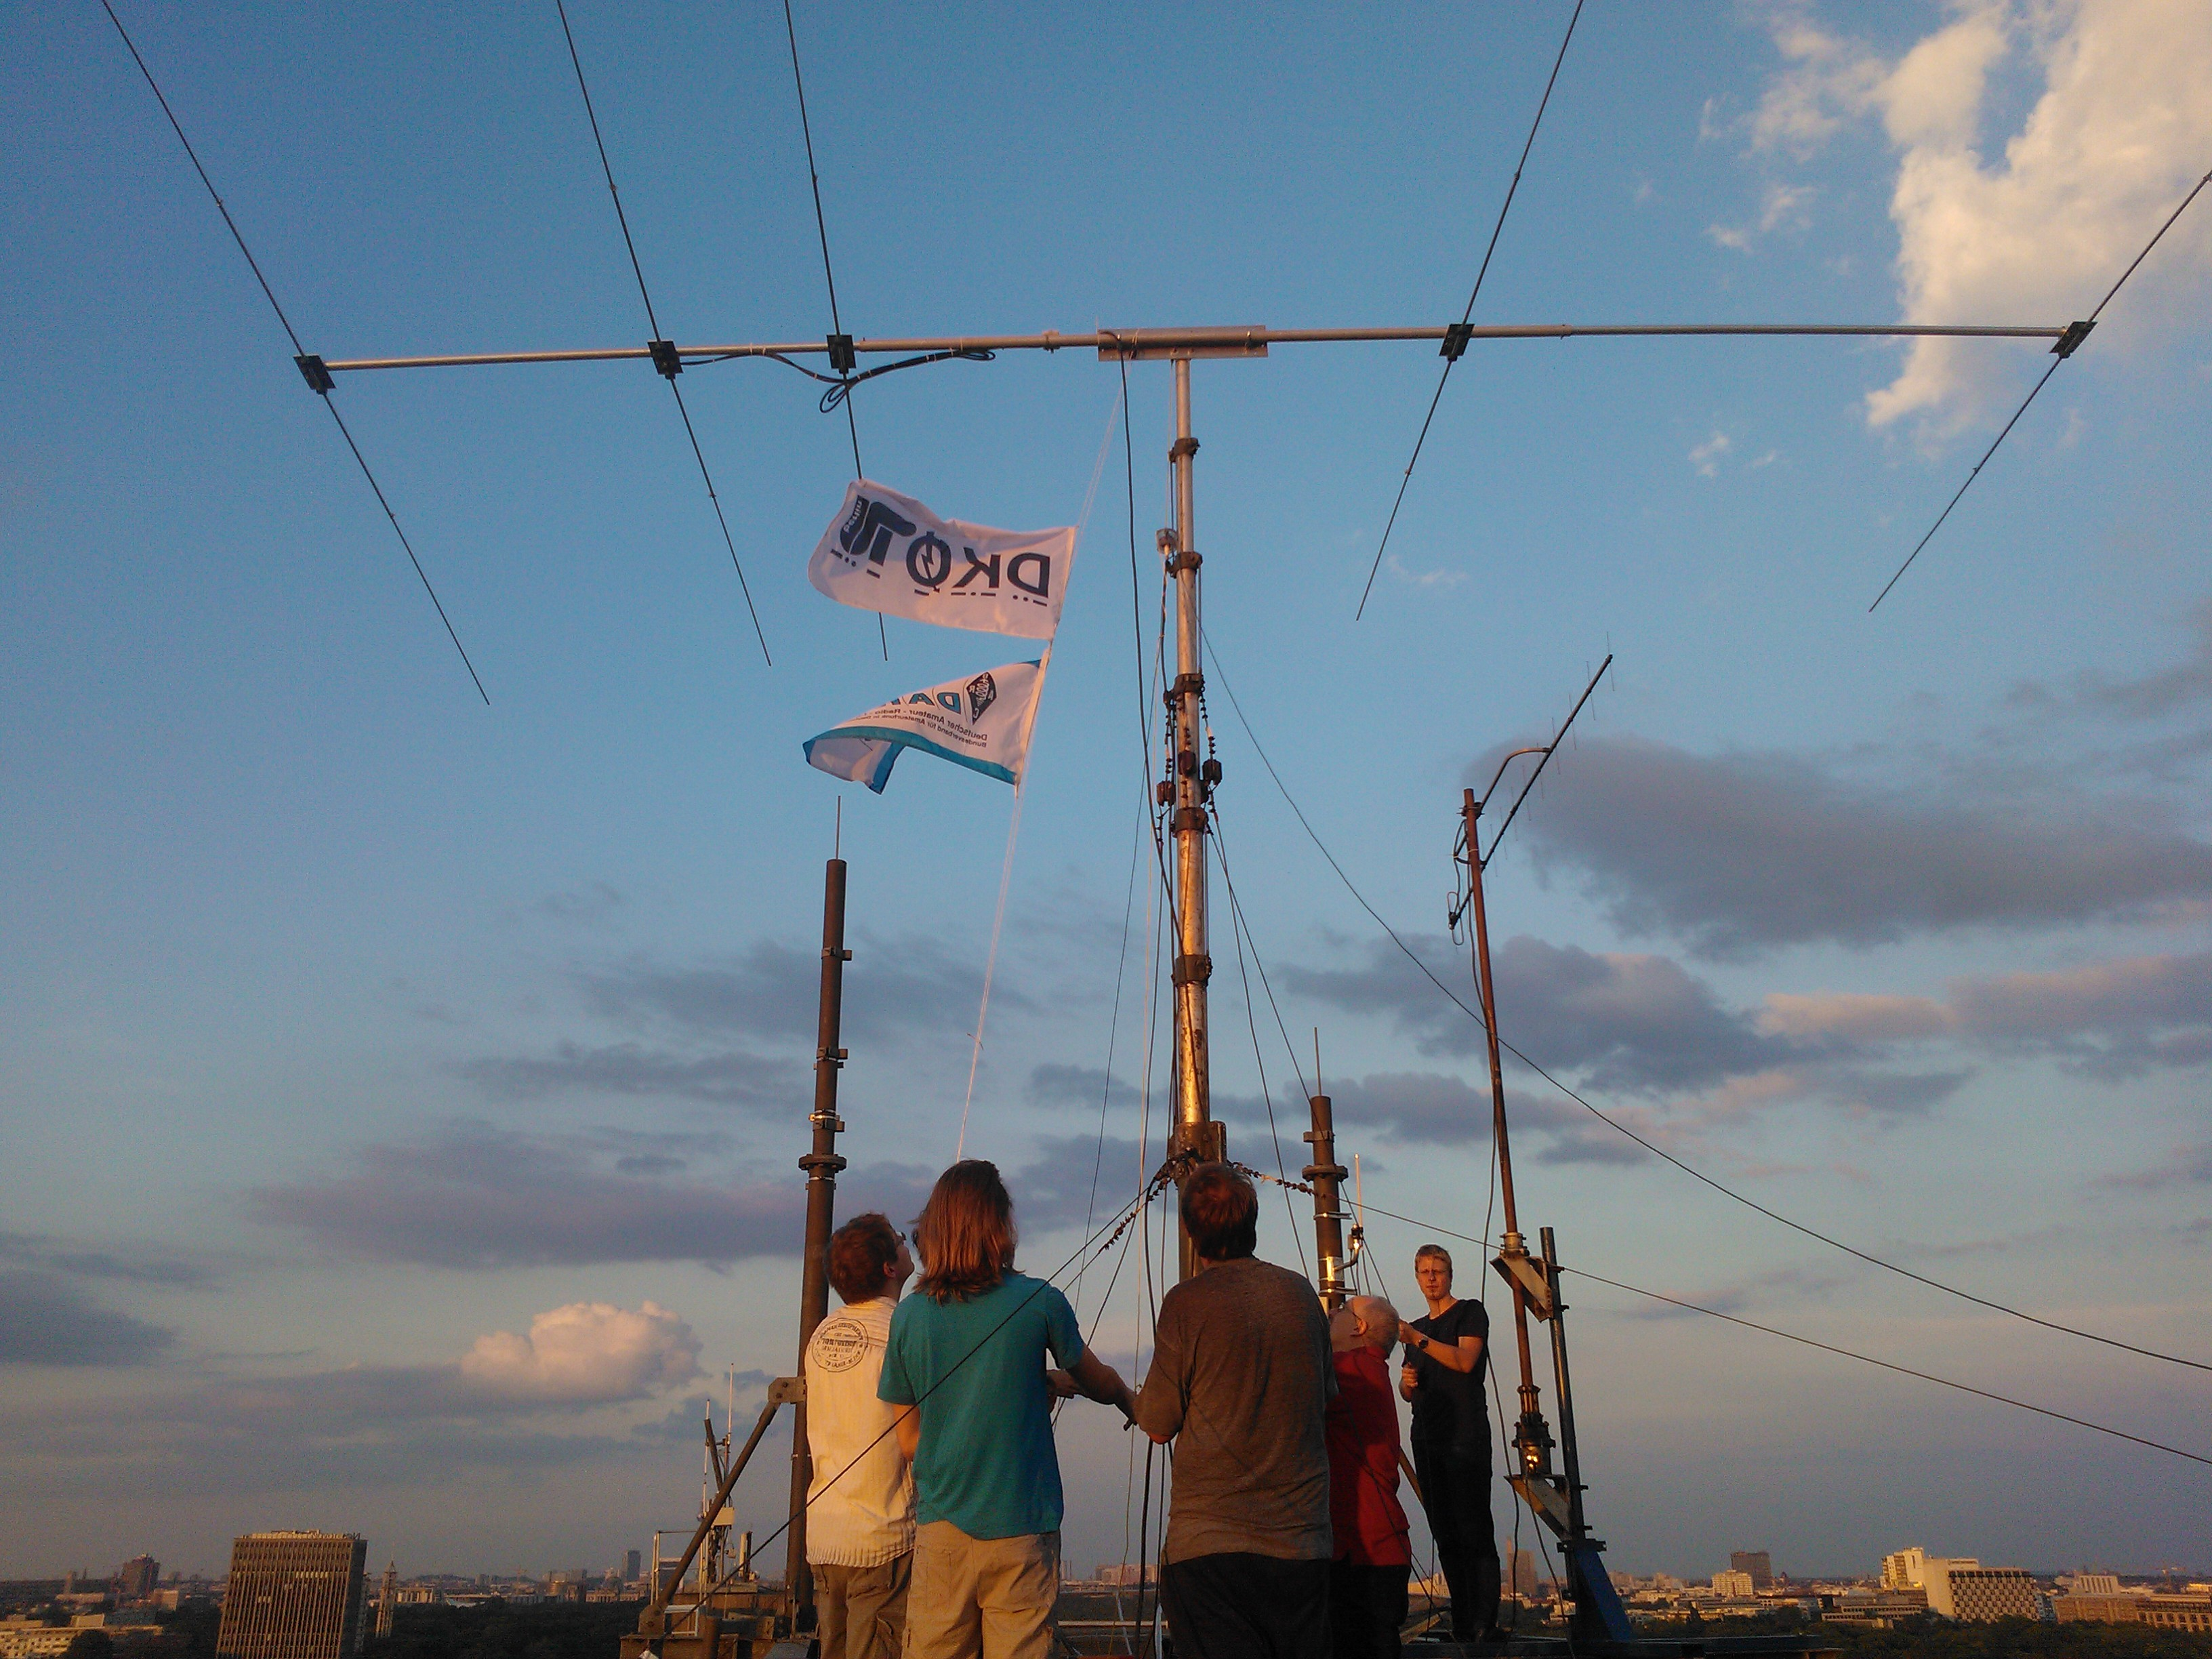
\includegraphics[width=.9\textwidth]{e11/yagi.jpg}
        \footnote{\tiny 10M Yagi bei DK0TU von DK9GD}
	\end{center}
\end{frame}

\begin{frame}
    \frametitle{Richtdiagramm Yagi}
    \begin{center}
        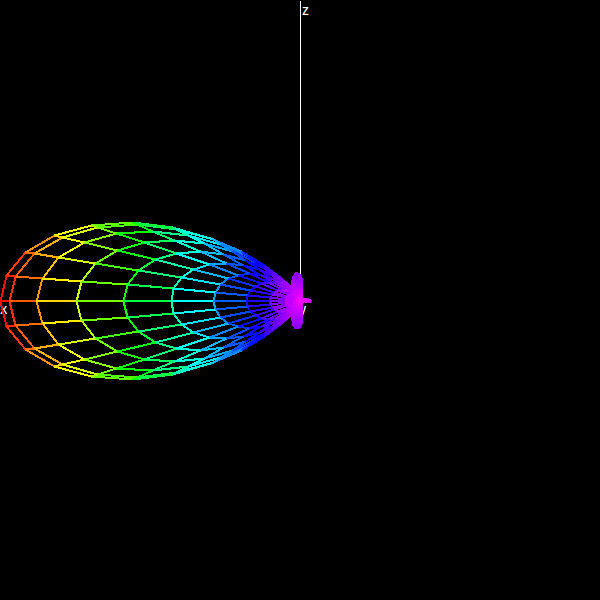
\includegraphics[width=0.7\textwidth]{e11/yagi_gain.png}
        \footnote{\tiny DK0TU 10m Yagi 28.1 MHz von DL2JAS Programm: EZNEC}
	\end{center}
\end{frame}

\section*{Groundplane}

\begin{frame}
    \frametitle{Groundplane}
    \begin{center}
        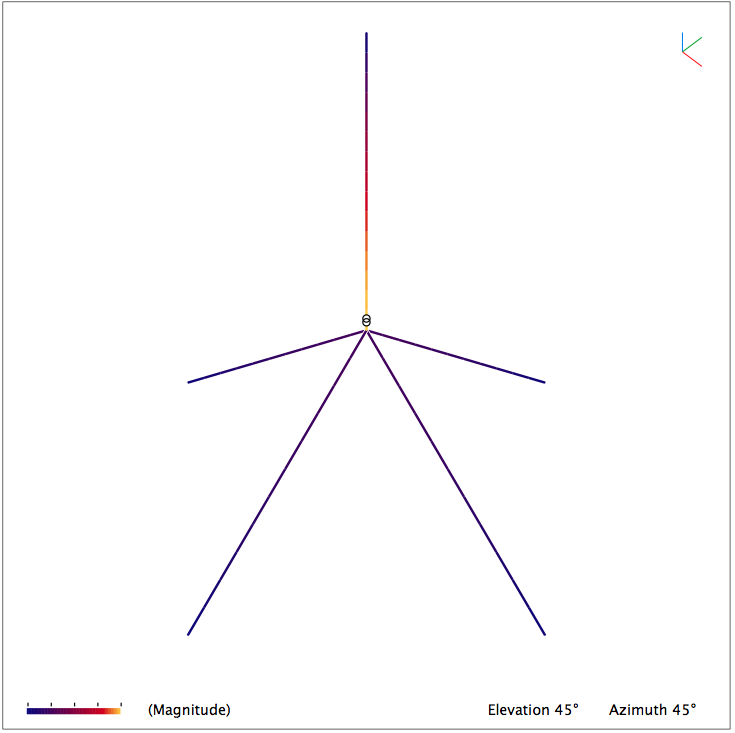
\includegraphics[width=0.7\textwidth]{e11/GP-DB4UM.png}
        \footnote{\tiny DB4UM mit cocoaNec 2.0}
	\end{center}
\end{frame}

\section*{Magnetic Loop}

\begin{frame}
    \frametitle{Magnetic Loop}
    \begin{center}
        \includegraphics[width=1\textwidth]{e11/Magloop.jpg}
        \footnote{\tiny Magloop bei DK0TU von DB4UM}
	\end{center}
\end{frame}

\section*{Polarisierung}

\begin{frame}
    \frametitle{Polarisierung}
    	\begin{itemize}
		\item Welche Antennen sind Vertikal, welche Horizontal Polarisiert?
		\item Wie ist die Antenne unten polarisiert?
    \end{itemize}
    \begin{center}
        \includegraphics[width=.4\textwidth]{e11/kreutzYagi.jpg}
        \footnote{\tiny DK0TU Fildday 2014 von DL7BUR}
	\end{center}
\end{frame}

\begin{frame}
    \frametitle{Welche Antenne ist was?}
    \begin{center}
        \includegraphics[width=1\textwidth]{e11/Abstrahl.png}
        \footnote{\tiny Bnetz-A Katalog Klasse E Prüfungsfrage TH202 }
	\end{center}
\end{frame}


\section*{Referenzen}

\begin{frame}
    \frametitle{Referenzen/Links}
    
    \footnotesize
    \begin{itemize}
        \item Moltrecht E 09: \\
              \url{http://www.dj4uf.de/lehrg/e11/e11.html}
        \item Strahlungsdiagramm (Youtube): \\
              \url{https://www.youtube.com/watch?v=gBqqp7rnZ64}
    \end{itemize}

\end{frame}

% Hier könnte noch eine Kontaktfolie stehen

\end{document}

